% !TeX program = xelatex
% Template báo cáo thực tập tốt nghiệp - Trường Đại học Đại Nam
% Biên dịch bằng XeLaTeX. Nên chạy 2 lần để cập nhật mục lục/danh mục.

\documentclass[12pt,a4paper,oneside]{extreport}

% Nạp cấu hình chung
% =====================================================
% settings.tex
% Cấu hình chung cho báo cáo
% Sinh viên chủ yếu sửa thông tin cá nhân ở mục 7.
% =====================================================

% =========================
% 1. CẤU HÌNH TIẾNG VIỆT VÀ FONT
% =========================
\usepackage{fontspec}
\IfFontExistsTF{Times New Roman}
  {\setmainfont{Times New Roman}}
  {\setmainfont{Tinos}}

\usepackage{polyglossia}
\setdefaultlanguage{vietnamese}

% =========================
% 2. CẤU HÌNH TRANG
% =========================
\usepackage[
    a4paper,
    left=3.0cm,
    right=1.5cm,
    top=2.0cm,
    bottom=2.0cm
]{geometry}

\usepackage{setspace}
\onehalfspacing

% Cỡ chữ mặc định của nội dung là 13pt. Các phần có quy định riêng
% bằng \fontsize trong tài liệu vẫn giữ nguyên cỡ chữ được chỉ định.
\makeatletter
\renewcommand{\normalsize}{%
    \@setfontsize\normalsize{13pt}{15.6pt}%
    \abovedisplayskip 13pt plus 3pt minus 7pt%
    \abovedisplayshortskip 0pt plus 4pt%
    \belowdisplayshortskip 6.5pt plus 3.5pt minus 3pt%
    \belowdisplayskip \abovedisplayskip
    \let\@listi\@listI
}
\makeatother
\normalsize

\usepackage{indentfirst}
\setlength{\parindent}{1.27cm}
\setlength{\parskip}{6pt}

% =========================
% 3. GÓI HỖ TRỢ
% =========================
\usepackage{graphicx}
\usepackage{float}
\usepackage{array}
\usepackage{longtable}
\usepackage{booktabs}
\usepackage{multirow}
\usepackage{tabularx}
\usepackage{caption}
\usepackage{amsmath, amssymb}
\usepackage{enumitem}
\setlist[itemize]{
    label=-,
    leftmargin=1.27cm,
    labelsep=0.5em
}
\usepackage{titlesec}
\usepackage{tocloft}
\usepackage{hyperref}
\usepackage{tikz}
\usetikzlibrary{arrows.meta,positioning,fit,backgrounds}
\usepackage{eso-pic}
\usepackage{fancyhdr}

% =========================
% 4. HYPERLINK
% =========================
\hypersetup{
    colorlinks=true,
    linkcolor=black,
    citecolor=black,
    urlcolor=blue
}

% Số trang đặt giữa phía trên; áp dụng cả cho trang mở đầu chương.
\setlength{\headheight}{17pt}
\pagestyle{fancy}
\fancyhf{}
\fancyhead[C]{\thepage}
\renewcommand{\headrulewidth}{0pt}
\fancypagestyle{plain}{
    \fancyhf{}
    \fancyhead[C]{\thepage}
    \renewcommand{\headrulewidth}{0pt}
}

% =========================
% 5. ĐÁNH SỐ HÌNH, BẢNG THEO CHƯƠNG
% =========================
\counterwithin{table}{chapter}
\counterwithin{figure}{chapter}
\renewcommand{\thetable}{\thechapter.\arabic{table}}
\renewcommand{\thefigure}{\thechapter.\arabic{figure}}

% Môi trường riêng cho sơ đồ để đánh số và lập danh mục độc lập.
\newfloat{sodo}{H}{los}[chapter]
\floatname{sodo}{Sơ đồ}
\renewcommand{\thesodo}{\thechapter.\arabic{sodo}}
\makeatletter
\newcommand{\l@sodo}[2]{%
    \begingroup
    \let\ReportOriginalNumberline\numberline
    \renewcommand{\numberline}[1]{%
        \ReportOriginalNumberline{Sơ đồ~##1}}%
    \@dottedtocline{1}{0pt}{2.8cm}{#1}{#2}%
    \endgroup
}
\makeatother

\captionsetup{
    font=normalsize,
    labelfont=normalfont,
    textfont=normalfont,
    labelsep=period,
    justification=centering
}
\captionsetup[table]{name=Bảng,position=top}
\captionsetup[figure]{name=Hình,position=bottom}
\captionsetup[sodo]{name=Sơ đồ,position=bottom}

\renewcommand{\listtablename}{BẢNG}
\renewcommand{\listfigurename}{HÌNH, SƠ ĐỒ}
\renewcommand{\contentsname}{MỤC LỤC}
\renewcommand{\bibname}{TÀI LIỆU THAM KHẢO}

% =========================
% 6. ĐỊNH DẠNG TIÊU ĐỀ CHƯƠNG, MỤC
% =========================
\titleformat{\chapter}
  [display]
  {\centering\bfseries\fontsize{14pt}{16pt}\selectfont}
  {Chương \thechapter}
  {0.3cm}
  {\MakeUppercase}

\titlespacing*{\chapter}{0pt}{0pt}{18pt}

\titleformat{\section}
  {\bfseries\fontsize{13pt}{15pt}\selectfont}
  {\thesection}
  {0.5em}
  {}

\titleformat{\subsection}
  {\bfseries\itshape\fontsize{13pt}{15pt}\selectfont}
  {\thesubsection}
  {0.5em}
  {}

\titleformat{\subsubsection}
  {\itshape\fontsize{13pt}{15pt}\selectfont}
  {\thesubsubsection}
  {0.5em}
  {}

\setcounter{secnumdepth}{3}
\setcounter{tocdepth}{3}

% =========================
% 7. ĐỊNH DẠNG MỤC LỤC
% =========================
\renewcommand{\cftchapfont}{\bfseries\fontsize{12pt}{14pt}\selectfont}
\renewcommand{\cftchappagefont}{\bfseries\fontsize{12pt}{14pt}\selectfont}
\renewcommand{\cftchappresnum}{CHƯƠNG~}
\renewcommand{\cftchapaftersnum}{.}
\setlength{\cftchapnumwidth}{2.5cm}
\renewcommand{\cftsecfont}{\bfseries\fontsize{12pt}{14pt}\selectfont}
\renewcommand{\cftsecpagefont}{\bfseries\fontsize{12pt}{14pt}\selectfont}
\renewcommand{\cftsecaftersnum}{.}
\renewcommand{\cftsubsecfont}{\itshape\fontsize{12pt}{14pt}\selectfont}
\renewcommand{\cftsubsecpagefont}{\fontsize{12pt}{14pt}\selectfont}
\renewcommand{\cftsubsecaftersnum}{.}
\renewcommand{\cftsubsubsecfont}{\fontsize{12pt}{14pt}\selectfont}
\renewcommand{\cftsubsubsecpagefont}{\fontsize{12pt}{14pt}\selectfont}
\renewcommand{\cftsubsubsecaftersnum}{.}
\renewcommand{\cftchapleader}{\cftdotfill{\cftdotsep}}
\setlength{\cftbeforechapskip}{6pt}

\renewcommand{\cfttoctitlefont}{\hfill\bfseries\fontsize{14pt}{16pt}\selectfont\MakeUppercase}
\renewcommand{\cftaftertoctitle}{\hfill}
\setlength{\cftbeforetoctitleskip}{0pt}
\setlength{\cftaftertoctitleskip}{18pt}

\makeatletter
\newcommand{\ReportListTable}[4]{%
    {\bfseries\fontsize{13pt}{14pt}\selectfont #1:\par}
    \vspace{6pt}
    \begingroup
    \fontsize{12pt}{13pt}\selectfont
    \renewcommand{\arraystretch}{1.5}
    \def\ReportListPrefix{#3}%
    \def\numberline##1{\ReportListPrefix~##1.\enspace}%
    \def\contentsline##1##2##3##4{##2\dotfill & ##3\\\hline}%
    \def\addvspace##1{}%
    \def\select@language##1{}%
    \makeatletter
    \noindent
    \begin{tabular}{|>{\raggedright\arraybackslash}p{\dimexpr\textwidth-3.5cm\relax}|>{\centering\arraybackslash}p{2.6cm}|}
        \hline
        \multicolumn{1}{|c|}{\bfseries #2} & \bfseries Trang \\
        \hline
        \@input{\jobname.#4}%
    \end{tabular}
    \par
    % Mở lại tệp danh mục để các caption phía sau tiếp tục ghi dữ liệu.
    \let\contentsline\@gobblefour
    \let\addvspace\@gobble
    \let\select@language\@gobble
    \@starttoc{#4}%
    \makeatother
    \endgroup
}

\newcommand{\CombinedLists}{%
    \chapter*{\fontsize{13pt}{14pt}\selectfont DANH MỤC CÁC BẢNG, SƠ ĐỒ, HÌNH}
    \addcontentsline{toc}{chapter}{DANH MỤC CÁC BẢNG, SƠ ĐỒ, HÌNH}
    \ReportListTable{BẢNG}{Tên bảng}{Bảng}{lot}
    \vspace{14pt}
    \ReportListTable{SƠ ĐỒ}{Tên sơ đồ}{Sơ đồ}{los}
    \vspace{14pt}
    \ReportListTable{HÌNH}{Tên hình}{Hình}{lof}
}
\makeatother

% =========================
% 8. THÔNG TIN SINH VIÊN/BÁO CÁO
% Sinh viên chỉ cần sửa phần này.
% =========================
\newcommand{\BoGiaoDuc}{BỘ GIÁO DỤC VÀ ĐÀO TẠO}
\newcommand{\TenTruong}{TRƯỜNG ĐẠI HỌC ĐẠI NAM}

\newcommand{\TenSinhVien}{HỌ VÀ TÊN SINH VIÊN}
\newcommand{\MaSinhVien}{...}
\newcommand{\KhoaHoc}{...}

\newcommand{\TenBaoCao}{PHÂN LOẠI TIN NHẮN RÁC (SPAM) BẰNG BIỂU DIỄN BAG-OF-WORDS/TF-IDF VÀ NAIVE BAYES}
\newcommand{\LoaiBaoCao}{BÀI TẬP LỚN HỌC PHẦN NHẬP MÔN HỌC MÁY}
\newcommand{\Nganh}{CÔNG NGHỆ THÔNG TIN}
\newcommand{\ChuyenNganh}{...}

\newcommand{\GiangVienHD}{ThS. Lê Thị Thùy Trang}

\newcommand{\DiaDiem}{HÀ NỘI}
\newcommand{\Nam}{2026}

% Logo trường. Có thể thay bằng file khác trong thư mục images/.
\newcommand{\LogoTruong}{images/logo-dai-nam.png}

% =========================
% 9. LỆNH CHƯƠNG KHÔNG ĐÁNH SỐ
% Dùng cho: Lời cam đoan, Lời cảm ơn, Mở đầu, Kết luận...
% =========================
\newcommand{\UnnumberedChapter}[1]{
    \chapter*{#1}
    \addcontentsline{toc}{chapter}{#1}
}

% Ghi nguồn ngay dưới bảng, hình hoặc sơ đồ khi sử dụng dữ liệu bên ngoài.
\newcommand{\Nguon}[1]{%
    \par\smallskip
    {\centering\itshape Nguồn: #1\par}
}

% Với môi trường sodo của gói float, caption luôn được dồn xuống cuối.
% Gộp nguồn vào caption để bảo đảm thứ tự hiển thị: tên sơ đồ, rồi đến nguồn.
\newcommand{\SodoCaption}[2]{%
    \caption[#1]{#1\\[3pt]\textit{Nguồn: #2}}%
}

% =========================
% 10. KHUNG TRANG BÌA
% =========================
\newcommand{\DrawCoverBorder}{
\AddToShipoutPictureBG*{
\begin{tikzpicture}[remember picture, overlay]
    \draw[line width=1pt]
        ([xshift=1.2cm,yshift=-1.2cm]current page.north west)
        rectangle
        ([xshift=-1.2cm,yshift=1.2cm]current page.south east);
\end{tikzpicture}
}
}

% =========================
% 11. TRÍCH DẪN
% \cite{khoa} -> [số], liên kết tới mục trong danh mục tài liệu tham khảo.
% =========================
\renewcommand{\cite}[1]{[\ref{bib:#1}]}

% Tránh tràn lề ở các dòng có lệnh \texttt dài không ngắt được.
\setlength{\emergencystretch}{3em}


\begin{document}

% =========================
% TRANG BÌA
% =========================
\pagenumbering{gobble}
% =====================================================
% cover.tex
% Hai trang bìa theo mẫu báo cáo thực tập tốt nghiệp
% =====================================================

% =========================
% TRANG BÌA 1
% =========================
\begin{titlepage}
\DrawCoverBorder
\centering

{\bfseries\fontsize{15pt}{18pt}\selectfont \BoGiaoDuc \par}
\vspace{0.3cm}
{\bfseries\fontsize{15pt}{18pt}\selectfont \TenTruong \par}

\vspace{0.8cm}

\includegraphics[width=0.27\textwidth]{\LogoTruong}

\vspace{1.0cm}

{\bfseries\fontsize{15pt}{18pt}\selectfont \TenSinhVien \par}

\vspace{0.3cm}

{\bfseries\fontsize{15pt}{18pt}\selectfont MSV: \MaSinhVien \par}

\vspace{1.3cm}

{\bfseries\fontsize{15pt}{18pt}\selectfont \TenBaoCao \par}

\vspace{1.8cm}

{\bfseries\fontsize{16pt}{18pt}\selectfont \LoaiBaoCao \par}

\vfill

{\bfseries\fontsize{14pt}{17pt}\selectfont \DiaDiem, NĂM \Nam \par}

\end{titlepage}

% =========================
% TRANG BÌA 2
% =========================
\begin{titlepage}
\DrawCoverBorder
\centering

{\bfseries\fontsize{15pt}{18pt}\selectfont \BoGiaoDuc \par}
\vspace{0.3cm}
{\bfseries\fontsize{15pt}{18pt}\selectfont \TenTruong \par}

\vspace{0.8cm}

\includegraphics[width=0.27\textwidth]{\LogoTruong}

\vspace{0.9cm}

{\bfseries\fontsize{15pt}{18pt}\selectfont \TenSinhVien \par}

\vspace{0.3cm}

{\bfseries\fontsize{15pt}{18pt}\selectfont MSV: \MaSinhVien, KHÓA: \KhoaHoc \par}

\vspace{1.0cm}

{\bfseries\fontsize{15pt}{18pt}\selectfont \TenBaoCao \par}

\vspace{1.4cm}

{\bfseries\fontsize{16pt}{18pt}\selectfont \LoaiBaoCao \par}

\vspace{0.4cm}

{\bfseries\fontsize{16pt}{18pt}\selectfont NGÀNH: \Nganh \par}

\vspace{0.4cm}

{\bfseries\fontsize{16pt}{18pt}\selectfont CHUYÊN NGÀNH: \ChuyenNganh \par}

\vspace{1.4cm}

{\bfseries\fontsize{14pt}{17pt}\selectfont GIẢNG VIÊN HƯỚNG DẪN: \GiangVienHD \par}

\vfill

{\bfseries\fontsize{14pt}{17pt}\selectfont \DiaDiem, NĂM \Nam \par}

\end{titlepage}


% =========================
% PHẦN ĐẦU BÁO CÁO
% =========================
\clearpage
\pagenumbering{roman}
\setcounter{page}{1}

\UnnumberedChapter{LỜI CAM ĐOAN}

Nhóm chúng tôi xin cam đoan báo cáo bài tập lớn học phần Nhập môn Học máy với đề tài \textit{``Phân loại tin nhắn rác (Spam) bằng biểu diễn Bag-of-Words/TF-IDF và Naive Bayes''} là kết quả nghiên cứu, thiết kế và thực nghiệm do chính nhóm thực hiện dưới sự hướng dẫn của giảng viên.

Toàn bộ số liệu, bảng biểu, hình vẽ trong báo cáo đều được sinh ra từ mã nguồn của nhóm trên bộ dữ liệu SMS Spam Collection (UCI) và có thể tái lập bằng các lệnh được mô tả trong Chương~4 và Phụ lục. Các tài liệu, thuật toán và công cụ của bên thứ ba được trích dẫn đầy đủ trong danh mục tài liệu tham khảo. Việc sử dụng công cụ trí tuệ nhân tạo hỗ trợ được khai báo minh bạch tại Phụ lục~3.

Nhóm xin chịu trách nhiệm về tính trung thực và chính xác của toàn bộ nội dung báo cáo.

\vspace{1cm}

\begin{flushright}
\begin{minipage}{8cm}
\centering
\textit{Hà Nội, ngày \ldots tháng \ldots năm \Nam}

\vspace{0.5cm}

\textbf{Đại diện nhóm}

\vspace{2cm}

\textbf{\TenSinhVien}
\end{minipage}
\end{flushright}

\UnnumberedChapter{LỜI CẢM ƠN}

Nhóm chúng tôi xin gửi lời cảm ơn chân thành tới Ban Giám hiệu Trường Đại học Đại Nam và Khoa Công nghệ thông tin đã tạo điều kiện học tập, nghiên cứu để nhóm hoàn thành học phần Nhập môn Học máy.

Nhóm đặc biệt cảm ơn giảng viên \GiangVienHD{} đã giao đề tài, cung cấp tiêu chí đánh giá rõ ràng, tận tình góp ý về cách đặt bài toán, cách đánh giá mô hình và cách trình bày kết quả. Những nhận xét của cô giúp nhóm tránh được các sai lầm phổ biến như rò rỉ dữ liệu hay chỉ dựa vào độ chính xác (accuracy) để kết luận.

Nhóm cũng xin cảm ơn các tác giả của bộ dữ liệu SMS Spam Collection và cộng đồng phát triển mã nguồn mở scikit-learn, pandas, NumPy, matplotlib, Streamlit đã cung cấp những công cụ chất lượng cao phục vụ cho bài tập lớn này.

Mặc dù đã nỗ lực hoàn thiện, báo cáo khó tránh khỏi thiếu sót. Nhóm kính mong nhận được ý kiến đóng góp của quý thầy cô để báo cáo và sản phẩm được hoàn thiện hơn.

\vspace{1cm}

\begin{flushright}
\begin{minipage}{8cm}
\centering
\textit{Hà Nội, ngày \ldots tháng \ldots năm \Nam}

\vspace{0.5cm}

\textbf{Đại diện nhóm}

\vspace{2cm}

\textbf{\TenSinhVien}
\end{minipage}
\end{flushright}

\UnnumberedChapter{KÍ HIỆU CÁC CỤM TỪ VIẾT TẮT}

\begin{longtable}{|p{4cm}|p{10cm}|}
\hline
\centering\textbf{TỪ VIẾT TẮT} & \centering\arraybackslash\textbf{TÊN ĐẦY ĐỦ} \\
\hline
\endhead
AUC & Area Under the Curve (diện tích dưới đường cong) \\
\hline
BoW & Bag-of-Words (túi từ) \\
\hline
CLI & Command-Line Interface (giao diện dòng lệnh) \\
\hline
CM & Confusion Matrix (ma trận nhầm lẫn) \\
\hline
CV & Cross-Validation (kiểm định chéo) \\
\hline
EDA & Exploratory Data Analysis (phân tích khám phá dữ liệu) \\
\hline
FN & False Negative (spam bị bỏ lọt) \\
\hline
FP & False Positive (tin hợp lệ bị chặn nhầm) \\
\hline
IDF & Inverse Document Frequency (nghịch đảo tần suất văn bản) \\
\hline
K-NN & K-Nearest Neighbors (K láng giềng gần nhất) \\
\hline
NB & Naive Bayes \\
\hline
NLP & Natural Language Processing (xử lý ngôn ngữ tự nhiên) \\
\hline
ROC & Receiver Operating Characteristic \\
\hline
SMS & Short Message Service (dịch vụ tin nhắn ngắn) \\
\hline
TF & Term Frequency (tần suất từ) \\
\hline
TF-IDF & Term Frequency -- Inverse Document Frequency \\
\hline
TN & True Negative (tin hợp lệ được giữ lại đúng) \\
\hline
TP & True Positive (spam bị chặn đúng) \\
\hline
UCI & University of California, Irvine (kho dữ liệu học máy) \\
\hline
\end{longtable}


% Danh mục bảng, sơ đồ, hình
\clearpage
\CombinedLists

% Mục lục
\clearpage
\tableofcontents

% Mở đầu
\clearpage
\UnnumberedChapter{LỜI MỞ ĐẦU}

Tin nhắn rác (spam) là một trong những vấn đề dai dẳng nhất của các kênh liên lạc số. Ngoài việc gây phiền toái, spam còn là phương tiện phát tán quảng cáo trái phép, lừa đảo trúng thưởng và thu thập thông tin cá nhân. Việc lọc spam tự động vì vậy là một bài toán phân loại văn bản kinh điển, đồng thời là bài toán thực tế có yêu cầu nghiệp vụ rõ ràng: \textit{chặn được nhiều spam nhưng hầu như không được chặn nhầm tin hợp lệ}.

Báo cáo này trình bày toàn bộ quy trình học máy giám sát cho bài toán phân loại tin nhắn SMS thành \textit{spam} và \textit{ham} (tin hợp lệ) trên bộ dữ liệu SMS Spam Collection do UCI công bố. Quy trình đi từ dữ liệu thô đến sản phẩm demo, gồm: phân tích khám phá dữ liệu, tiền xử lý văn bản, biểu diễn đặc trưng bằng Bag-of-Words và TF-IDF, huấn luyện ba thuật toán (Multinomial Naive Bayes, K-NN, Decision Tree), đánh giá bằng các thước đo phù hợp với dữ liệu mất cân bằng, phân tích lỗi và đề xuất ứng dụng.

\textbf{Mục tiêu của báo cáo:}
\begin{itemize}
    \item Xây dựng pipeline phân loại spam hoàn chỉnh, có baseline, có thí nghiệm đối chứng (ablation), \textit{không rò rỉ dữ liệu} và \textit{tái lập được}.
    \item Chứng minh bằng số liệu tác động của từng quyết định thiết kế (BoW so với TF-IDF, unigram so với bigram, thuật toán, tiền xử lý) lên chất lượng mô hình.
    \item Đánh giá mô hình một cách trung thực: nêu rõ phương sai do cách chia dữ liệu, kết quả kiểm tra rò rỉ/học thuộc và các hạn chế của dữ liệu.
    \item Diễn giải lỗi và đưa ra khuyến nghị ứng dụng dựa trên bằng chứng.
\end{itemize}

\textbf{Bố cục báo cáo} gồm bảy chương: Chương~1 giới thiệu bài toán và dữ liệu; Chương~2 trình bày cơ sở lý thuyết; Chương~3 phân tích khám phá dữ liệu, tiền xử lý và biểu diễn đặc trưng; Chương~4 mô tả thiết kế pipeline và thiết lập thí nghiệm; Chương~5 trình bày kết quả và so sánh; Chương~6 phân tích lỗi và diễn giải mô hình; Chương~7 đề xuất ứng dụng thực tế và mô tả sản phẩm demo. Phần Kết luận tổng kết, nêu hạn chế và hướng phát triển. Các phụ lục cung cấp thông tin tái lập, phân công công việc và khai báo sử dụng công cụ AI.


% =========================
% NỘI DUNG CHÍNH
% Mỗi chương là một file riêng trong thư mục chapters/
% =========================
\clearpage
\pagenumbering{arabic}
\setcounter{page}{1}
\chapter{GIỚI THIỆU BÀI TOÁN VÀ DỮ LIỆU}

\section{Bối cảnh và ý nghĩa thực tiễn}

Tin nhắn SMS vẫn là kênh liên lạc có độ phủ rộng nhất, không phụ thuộc vào kết nối Internet hay một ứng dụng cụ thể. Chính vì vậy SMS là mục tiêu thường xuyên của quảng cáo trái phép, lừa đảo trúng thưởng, dụ dỗ đăng ký dịch vụ tính cước và giả mạo thương hiệu. Một bộ lọc spam hiệu quả mang lại lợi ích ở ba phía:

\begin{itemize}
    \item \textbf{Người dùng}: giảm phiền toái và giảm rủi ro bị lừa đảo.
    \item \textbf{Nhà mạng và nền tảng nhắn tin}: bảo vệ uy tín dịch vụ, giảm chi phí khiếu nại.
    \item \textbf{Xã hội}: hạn chế các chiến dịch lừa đảo quy mô lớn.
\end{itemize}

Từ góc độ học máy, đây là bài toán \textit{phân loại văn bản nhị phân} với hai đặc điểm đáng chú ý: (i) dữ liệu mất cân bằng lớp (spam chiếm tỉ lệ thấp), và (ii) hai loại lỗi có chi phí rất khác nhau. Chặn nhầm một tin hợp lệ (mã OTP, thông báo từ ngân hàng, tin của người thân) gây hậu quả nặng hơn nhiều so với để lọt một tin quảng cáo. Hai đặc điểm này quyết định cách chọn thước đo đánh giá trong suốt báo cáo.

\section{Phát biểu bài toán}

Cho một tin nhắn $d$ là chuỗi ký tự, cần học hàm
\[
f:\ d \mapsto \hat{y}\in\{0,1\},
\]
trong đó $\hat{y}=1$ là \textit{spam} và $\hat{y}=0$ là \textit{ham} (tin hợp lệ). Báo cáo quy ước \textbf{spam là lớp dương}, vì vậy Precision, Recall và F1 được tính cho lớp spam; đây là lựa chọn bắt buộc để các thước đo có ý nghĩa nghiệp vụ trên dữ liệu mất cân bằng.

Bài toán được giải theo hướng học có giám sát cổ điển: biểu diễn văn bản thành vector đặc trưng thưa (Bag-of-Words hoặc TF-IDF), sau đó huấn luyện bộ phân loại. Phạm vi của báo cáo \textit{không} bao gồm các mô hình mạng nơ-ron sâu hay mô hình ngôn ngữ lớn; các hướng đó chỉ được thảo luận ở phần hướng phát triển.

\section{Bộ dữ liệu SMS Spam Collection}

\subsection{Nguồn và thành phần}

Báo cáo sử dụng đúng bộ dữ liệu giảng viên chỉ định: \textit{SMS Spam Collection v.1} do Almeida, Gómez Hidalgo và Yamakami công bố, được phân phối qua kho dữ liệu UCI Machine Learning Repository \cite{almeida2011}\cite{uci_sms}. Bộ dữ liệu gồm 5\,574 tin nhắn tiếng Anh, mỗi tin có một nhãn \textit{ham} hoặc \textit{spam}, lưu ở dạng tệp văn bản phân tách bằng ký tự tab (\texttt{nhãn<TAB>nội dung}), không có dòng tiêu đề.

Theo tài liệu đi kèm bộ dữ liệu, corpus được ghép từ bốn nguồn khác nhau (Bảng~\ref{tab:nguon-du-lieu}).

\begin{table}[H]
\centering
\caption{Thành phần nguồn của bộ dữ liệu SMS Spam Collection}
\label{tab:nguon-du-lieu}
\begin{tabular}{|p{6.2cm}|c|c|p{3.2cm}|}
\hline
\textbf{Nguồn} & \textbf{Ham} & \textbf{Spam} & \textbf{Ghi chú} \\
\hline
Diễn đàn Grumbletext (Vương quốc Anh) & -- & 425 & Trích thủ công từ các bài đăng khiếu nại \\
\hline
Luận án tiến sĩ của C. Tagg (2009) & 450 & -- & SMS đời thường \\
\hline
NUS SMS Corpus (Singapore) & 3\,375 & -- & Phần lớn từ sinh viên \\
\hline
SMS Spam Corpus v.0.1 Big & 1\,002 & 322 & Corpus trước đó của nhóm tác giả \\
\hline
\textbf{Tổng} & \textbf{4\,827} & \textbf{747} & \textbf{5\,574 tin} \\
\hline
\end{tabular}
\Nguon{Tài liệu \texttt{readme} đi kèm bộ dữ liệu; nhóm tổng hợp}
\end{table}

\subsection{Định dạng và đặc điểm ngôn ngữ}

Các tin nhắn chứa nhiều đặc trưng của văn bản SMS thực tế: viết tắt (\textit{u}, \textit{ur}, \textit{2day}, \textit{4}), lỗi chính tả, biểu tượng cảm xúc, ký tự đặc biệt (\textit{£}, \textit{\&lt;\#\&gt;}) và số điện thoại hoặc đầu số dịch vụ. Đây là lý do việc làm sạch văn bản cần được thiết kế thận trọng thay vì xóa máy móc mọi ký tự không phải chữ cái (xem Mục~\ref{sec:tien-xu-ly}).

\section{Giả định và giới hạn của dữ liệu}

Nhóm chủ động nêu các giới hạn của bộ dữ liệu ngay từ đầu vì chúng ảnh hưởng trực tiếp tới mức độ tin cậy của mọi kết luận ở các chương sau.

\begin{enumerate}[label=(\arabic*)]
    \item \textbf{Chỉ có tiếng Anh.} Mô hình học trên từ vựng tiếng Anh, vì vậy không áp dụng được cho tin nhắn tiếng Việt nếu không huấn luyện lại bằng dữ liệu tiếng Việt.
    \item \textbf{Dữ liệu cũ và nhỏ.} Corpus được thu thập chủ yếu trước năm 2012, quy mô khoảng năm nghìn tin. Hình thức spam hiện nay (liên kết rút gọn, giả mạo ngân hàng, mã QR) khác đáng kể.
    \item \textbf{Ham và spam đến từ các nguồn khác nhau.} Phần lớn ham là tin của sinh viên Singapore, phần lớn spam đến từ khiếu nại của người dùng Anh. Mô hình có thể học phần nào các khác biệt về \textit{nguồn} (phương ngữ, định dạng) thay vì chỉ học khác biệt về \textit{bản chất spam}. Do đó con số kết quả chỉ mô tả corpus này, không chứng minh khả năng tổng quát hóa sang SMS hiện đại.
    \item \textbf{Có tin trùng lặp.} Corpus chứa 414 tin có nội dung trùng với tin khác; cách xử lý được nêu ở Mục~\ref{sec:eda-trung-lap}.
    \item \textbf{Nhãn được giả định là đúng.} Nhóm không kiểm định lại nhãn thủ công; nhãn có thể chứa nhiễu nhỏ.
\end{enumerate}

\section{Mục tiêu và đóng góp của nhóm}

Mục tiêu kỹ thuật của bài tập lớn:

\begin{enumerate}[label=(\arabic*)]
    \item Xây dựng pipeline từ dữ liệu thô đến đánh giá và demo, tổ chức mã nguồn theo mô-đun để dễ mở rộng.
    \item Thiết lập baseline và tối thiểu hai phương án thực nghiệm có ý nghĩa; so sánh BoW với TF-IDF, unigram với bigram, và ba thuật toán.
    \item Chạy thí nghiệm đối chứng (ablation) cho các bước tiền xử lý để có bằng chứng định lượng cho từng quyết định.
    \item Đánh giá đa chiều (Accuracy, Precision, Recall, F1 của lớp spam, ROC-AUC, ma trận nhầm lẫn), kèm kiểm tra rò rỉ dữ liệu và học thuộc.
    \item Phân tích lỗi cụ thể và đề xuất cải tiến dựa trên các lỗi quan sát được.
\end{enumerate}

Các đóng góp chính của nhóm gồm: (i) một thư viện Python \texttt{spam\_filter} có cấu hình tập trung, 41 bài kiểm thử tự động và giao diện dòng lệnh; (ii) bộ thí nghiệm E0--E6 có bảng log tham số; (iii) bộ kiểm tra rò rỉ/học thuộc/baseline đơn giản; (iv) ứng dụng web demo bằng Streamlit.

\section{Tiêu chí thành công}

Do đặc thù nghiệp vụ, nhóm đặt tiêu chí thành công theo thứ tự ưu tiên như sau:

\begin{table}[H]
\centering
\caption{Tiêu chí đánh giá thành công của hệ thống lọc spam}
\label{tab:tieu-chi}
\begin{tabular}{|c|p{3.6cm}|p{9cm}|}
\hline
\textbf{STT} & \textbf{Tiêu chí} & \textbf{Lý do} \\
\hline
1 & Precision của lớp spam cao & Chặn nhầm tin hợp lệ (FP) gây hậu quả nặng nhất. \\
\hline
2 & Recall của lớp spam cao & Bỏ lọt spam (FN) gây phiền toái, nhưng người dùng vẫn đọc được tin. \\
\hline
3 & F1 của lớp spam & Một con số tổng hợp để so sánh các phương án và chọn mô hình. \\
\hline
4 & Kết quả ổn định, không rò rỉ & Con số phải đáng tin: không do trùng dữ liệu, học thuộc hay may mắn khi chia. \\
\hline
\end{tabular}
\Nguon{Nhóm xây dựng}
\end{table}

Accuracy \textit{không} được dùng làm tiêu chí chính. Lý do được phân tích định lượng ở Mục~\ref{sec:accuracy-lua-doi}.

\chapter{CƠ SỞ LÝ THUYẾT}

Chương này trình bày các kiến thức nền tảng được sử dụng trong báo cáo (có thể xem thêm giáo trình tiếng Việt \cite{tiep2018}), với trọng tâm là những điểm giải thích \textit{vì sao} mỗi lựa chọn thiết kế ở các chương sau là hợp lý.

\section{Biểu diễn văn bản dạng vector}

Các thuật toán học máy làm việc với vector số, vì vậy văn bản cần được chuyển thành vector đặc trưng. Gọi $V$ là từ vựng (tập các token) xây dựng từ \textit{tập huấn luyện}; mỗi văn bản $d$ được biểu diễn bởi vector $\mathbf{x}\in\mathbb{R}^{|V|}$.

\subsection{Bag-of-Words (BoW)}

Trong mô hình túi từ, thành phần $x_w$ là số lần từ $w$ xuất hiện trong $d$, bỏ qua thứ tự từ. Ưu điểm là đơn giản, nhanh và kết hợp tự nhiên với Multinomial Naive Bayes. Nhược điểm là các từ rất phổ biến (\textit{to}, \textit{you}, \textit{the}) có trọng số lớn dù ít mang thông tin phân biệt.

\subsection{TF-IDF}

TF-IDF điều chỉnh tần suất thô bằng độ hiếm của từ trong toàn corpus. Dựa trên ý tưởng của Spärck Jones \cite{sparckjones1972} và với cài đặt mặc định của scikit-learn \cite{scikit-learn} (làm mượt IDF):
\begin{equation}
\mathrm{idf}(w)=\ln\frac{1+n}{1+\mathrm{df}(w)}+1,\qquad
x_w=\mathrm{tf}(w,d)\cdot\mathrm{idf}(w),
\end{equation}
trong đó $n$ là số văn bản huấn luyện và $\mathrm{df}(w)$ là số văn bản chứa $w$. Sau đó vector được chuẩn hóa theo chuẩn $L_2$, nên độ dài tin nhắn ít ảnh hưởng đến so sánh. Từ xuất hiện ở nhiều văn bản có IDF thấp, từ hiếm nhưng đặc trưng (\textit{prize}, \textit{claim}) có IDF cao.

\subsection{N-gram và các tham số từ vựng}

\textit{N-gram} là chuỗi $n$ token liên tiếp. Unigram $(1,1)$ chỉ xét từ đơn; \textit{bigram} $(1,2)$ bổ sung cụm hai từ như \textit{``to claim''}, \textit{``have won''}, \textit{``call now''}, giữ lại một phần thông tin ngữ cảnh mà BoW bỏ mất. Cái giá là từ vựng tăng mạnh và vector thưa hơn. Hai tham số kiểm soát kích thước từ vựng:
\begin{itemize}
    \item \texttt{min\_df}: bỏ các n-gram xuất hiện trong ít hơn một ngưỡng văn bản, giảm nhiễu và chi phí tính toán;
    \item \texttt{max\_df}: bỏ các n-gram xuất hiện trong quá tỉ lệ văn bản cho trước (gần như từ dừng).
\end{itemize}

\section{Các thuật toán phân loại}

\subsection{Multinomial Naive Bayes}

Mô hình sự kiện đa thức cho phân loại văn bản được McCallum và Nigam \cite{mccallum1998} so sánh chi tiết với mô hình Bernoulli, và được trình bày hệ thống trong giáo trình của Manning và cộng sự \cite{manning2008}; Rennie và cộng sự \cite{rennie2003} phân tích các giả định yếu của nó và các hiệu chỉnh khi dùng với TF-IDF.

Theo định lý Bayes, xác suất hậu nghiệm của lớp $c$ cho văn bản $d$ là $P(c\mid d)\propto P(c)P(d\mid c)$. Giả định ``ngây thơ'' coi các từ độc lập có điều kiện khi biết lớp:
\begin{equation}
P(c\mid d)\ \propto\ P(c)\prod_{w\in V}P(w\mid c)^{x_w}.
\end{equation}
Với làm mượt Laplace/Lidstone tham số $\alpha$:
\begin{equation}
P(w\mid c)=\frac{N_{wc}+\alpha}{N_c+\alpha|V|},
\end{equation}
trong đó $N_{wc}$ là tổng giá trị đặc trưng của từ $w$ trên các văn bản lớp $c$ và $N_c=\sum_{w}N_{wc}$. Thực tế dự đoán được tính trong không gian logarit để tránh tràn số dưới:
\begin{equation}
\hat{c}=\arg\max_c\Big[\ln P(c)+\sum_{w}x_w\ln P(w\mid c)\Big].
\end{equation}

\textbf{Vì sao hợp với văn bản?} (i) Vector văn bản có hàng chục nghìn chiều nhưng rất thưa, trong khi số tham số cần ước lượng của NB chỉ tỉ lệ với $|V|$ nên ít bị quá khớp trên dữ liệu nhỏ; (ii) huấn luyện chỉ là đếm, rất nhanh; (iii) mô hình \textit{khả diễn giải} vì $\ln P(w\mid\mathrm{spam})-\ln P(w\mid\mathrm{ham})$ cho biết từ nào đẩy tin về phía spam. Giả định độc lập rõ ràng không đúng với ngôn ngữ, nhưng với mục đích \textit{phân loại} (chỉ cần xếp hạng đúng lớp), sai lệch này thường ít gây hại; còn xác suất đầu ra thường kém hiệu chuẩn (quá tự tin), nên ngưỡng quyết định cần được hiệu chỉnh thay vì mặc định 0,5.

\textbf{Vai trò của $\alpha$.} $\alpha$ nhỏ làm mô hình tin vào từng từ hiếm hơn (phương sai cao), $\alpha$ lớn kéo mọi xác suất về gần nhau (thiên lệch cao). Với từ vựng bigram lớn, $\alpha$ lớn làm loãng tín hiệu của các cụm hiếm nhưng quyết định; điều này được kiểm chứng ở Mục~\ref{sec:nhay-tham-so}.

\subsection{K láng giềng gần nhất (K-NN)}

K-NN dự đoán lớp của $d$ bằng đa số nhãn của $k$ văn bản huấn luyện gần nhất. Với vector TF-IDF đã chuẩn hóa $L_2$, khoảng cách cosine
\begin{equation}
d_{\cos}(\mathbf{x},\mathbf{z})=1-\frac{\mathbf{x}\cdot\mathbf{z}}{\lVert\mathbf{x}\rVert\,\lVert\mathbf{z}\rVert}
\end{equation}
là lựa chọn chuẩn cho văn bản vì không phụ thuộc độ dài. K-NN không có giai đoạn huấn luyện thực sự (``học lười''), chi phí dự đoán tỉ lệ với kích thước tập huấn luyện, và chịu ảnh hưởng của ``lời nguyền số chiều'': trong không gian hàng chục nghìn chiều, khoảng cách giữa các điểm có xu hướng đồng đều, làm mất khả năng phân biệt.

\subsection{Cây quyết định (Decision Tree)}

Cây quyết định chia đệ quy không gian đặc trưng bằng các điều kiện dạng $x_w\le\tau$, tại mỗi nút chọn phép chia làm giảm độ tạp Gini nhiều nhất:
\begin{equation}
G=1-\sum_{k}p_k^2 .
\end{equation}
Cây có tính diễn giải cao nhưng dễ quá khớp; các siêu tham số \texttt{max\_depth} và \texttt{min\_samples\_leaf} dùng để giới hạn độ phức tạp. Trên vector văn bản thưa nhiều chiều, một cây đơn thường chỉ dựa vào vài từ khóa nên khó đạt Recall cao.

\section{Thước đo đánh giá}

Với spam là lớp dương, ma trận nhầm lẫn gồm TP (spam bị chặn đúng), FP (ham bị chặn nhầm), FN (spam bị bỏ lọt) và TN (ham được giữ lại đúng). Khi đó:
\begin{align}
\mathrm{Accuracy}&=\frac{TP+TN}{TP+TN+FP+FN},\\
\mathrm{Precision}&=\frac{TP}{TP+FP},\qquad
\mathrm{Recall}=\frac{TP}{TP+FN},\\
F_1&=\frac{2\cdot\mathrm{Precision}\cdot\mathrm{Recall}}{\mathrm{Precision}+\mathrm{Recall}}.
\end{align}

\begin{itemize}
    \item \textbf{Precision} đo trong số tin bị chặn thì bao nhiêu thực sự là spam: nó phản ánh rủi ro \textit{chặn nhầm}.
    \item \textbf{Recall} đo trong số spam thật thì bắt được bao nhiêu: nó phản ánh rủi ro \textit{bỏ lọt}.
    \item \textbf{F1} là trung bình điều hòa của hai đại lượng trên, bị kéo xuống nếu một trong hai thấp.
    \item \textbf{ROC-AUC} là xác suất mô hình xếp một spam ngẫu nhiên cao điểm hơn một ham ngẫu nhiên; thước đo này không phụ thuộc ngưỡng quyết định.
\end{itemize}

\section{Kiểm định chéo và rò rỉ dữ liệu}

\textbf{Kiểm định chéo phân tầng $K$-fold} chia tập huấn luyện thành $K$ phần giữ nguyên tỉ lệ lớp; lần lượt dùng một phần để kiểm định và $K-1$ phần để huấn luyện, rồi lấy trung bình. Báo cáo dùng $K=5$ và dùng \textbf{F1 của lớp spam qua CV trên tập huấn luyện} để \textit{chọn mô hình}, nhờ vậy tập kiểm tra (test) chỉ được dùng để báo cáo cuối cùng chứ không tham gia vào việc chọn.

\textbf{Rò rỉ dữ liệu (data leakage)} xảy ra khi thông tin từ tập kiểm tra ``lọt'' vào quá trình huấn luyện, làm kết quả đẹp một cách giả tạo. Hai nguồn rò rỉ thường gặp với văn bản là: (i) \textit{fit vectorizer trên toàn bộ dữ liệu} (từ vựng và IDF bị tính cả từ tập test), và (ii) \textit{tin trùng lặp nằm ở cả hai tập}. Cách phòng ngừa của nhóm: bọc toàn bộ chuỗi làm sạch, vector hóa và mô hình trong một \texttt{Pipeline} của scikit-learn, nhờ đó mọi bước học từ dữ liệu chỉ được \texttt{fit} trên phần huấn luyện (kể cả trong từng fold của CV), và bỏ trùng lặp \textit{trước} khi chia.

\chapter{KHÁM PHÁ DỮ LIỆU, TIỀN XỬ LÝ VÀ BIỂU DIỄN ĐẶC TRƯNG}

\section{Phân tích khám phá dữ liệu (EDA)}

\subsection{Kích thước, kiểu dữ liệu và giá trị thiếu}

Sau khi đọc tệp với dấu phân tách tab và tắt cơ chế xử lý ngoặc kép (tin nhắn có thể chứa ký tự \texttt{"} không phải dấu bao trường), bộ dữ liệu có 5\,574 dòng và hai cột: \texttt{label} (chuỗi \textit{ham}/\textit{spam}) và \texttt{text} (chuỗi). Không có giá trị thiếu ở cả hai cột. Nhãn được mã hóa \texttt{ham}$\to0$, \texttt{spam}$\to1$ để spam là lớp dương.

\subsection{Tin nhắn trùng lặp}
\label{sec:eda-trung-lap}

Corpus gốc chứa \textbf{414 tin có nội dung trùng với một tin khác} (sau khi cắt khoảng trắng đầu/cuối), gồm 309 tin ham và 105 tin spam. Không có trường hợp cùng nội dung nhưng khác nhãn. Việc trùng lặp gây hai tác hại: làm sai lệch phân phối thật của dữ liệu, và nếu để cả hai bản sao ở hai phía của phép chia thì mô hình chỉ cần \textit{ghi nhớ} là đạt điểm cao trên test (rò rỉ). Nhóm \textbf{bỏ các bản trùng trước khi chia}, giữ lại một bản. Kết quả còn \textbf{5\,160 tin} (4\,518 ham, 642 spam).

\begin{table}[H]
\centering
\caption{Quy mô dữ liệu trước và sau khi loại bản trùng}
\label{tab:quy-mo}
\begin{tabular}{|p{5.4cm}|c|c|c|}
\hline
\textbf{Giai đoạn} & \textbf{Ham} & \textbf{Spam} & \textbf{Tổng} \\
\hline
Corpus gốc & 4\,827 & 747 & 5\,574 \\
\hline
Số tin trùng bị loại & 309 & 105 & 414 \\
\hline
Sau khi loại bản trùng & 4\,518 & 642 & 5\,160 \\
\hline
Tập huấn luyện (80\%) & 3\,614 & 514 & 4\,128 \\
\hline
Tập kiểm tra (20\%) & 904 & 128 & 1\,032 \\
\hline
\end{tabular}
\Nguon{Nhóm tính từ bộ dữ liệu SMS Spam Collection}
\end{table}

Phép chia $80/20$ có phân tầng theo nhãn nên tỉ lệ spam ở hai tập gần như bằng nhau (12,5\% ở tập huấn luyện và 12,4\% ở tập kiểm tra).

\subsection{Mất cân bằng lớp}
\label{sec:accuracy-lua-doi}

Spam chỉ chiếm \textbf{12,4\%} dữ liệu sau khi khử trùng lặp (Hình~\ref{fig:eda-balance}, bên trái). Hệ quả quan trọng: một ``mô hình'' luôn trả lời \textit{ham} sẽ đạt Accuracy $=904/1032\approx 87{,}6\%$ trên tập kiểm tra nhưng có Recall của lớp spam bằng 0; nó hoàn toàn vô dụng. Vì vậy Accuracy \textbf{không đủ} để đánh giá và báo cáo luôn kèm Precision, Recall và F1 của lớp spam.

\begin{figure}[H]
    \centering
    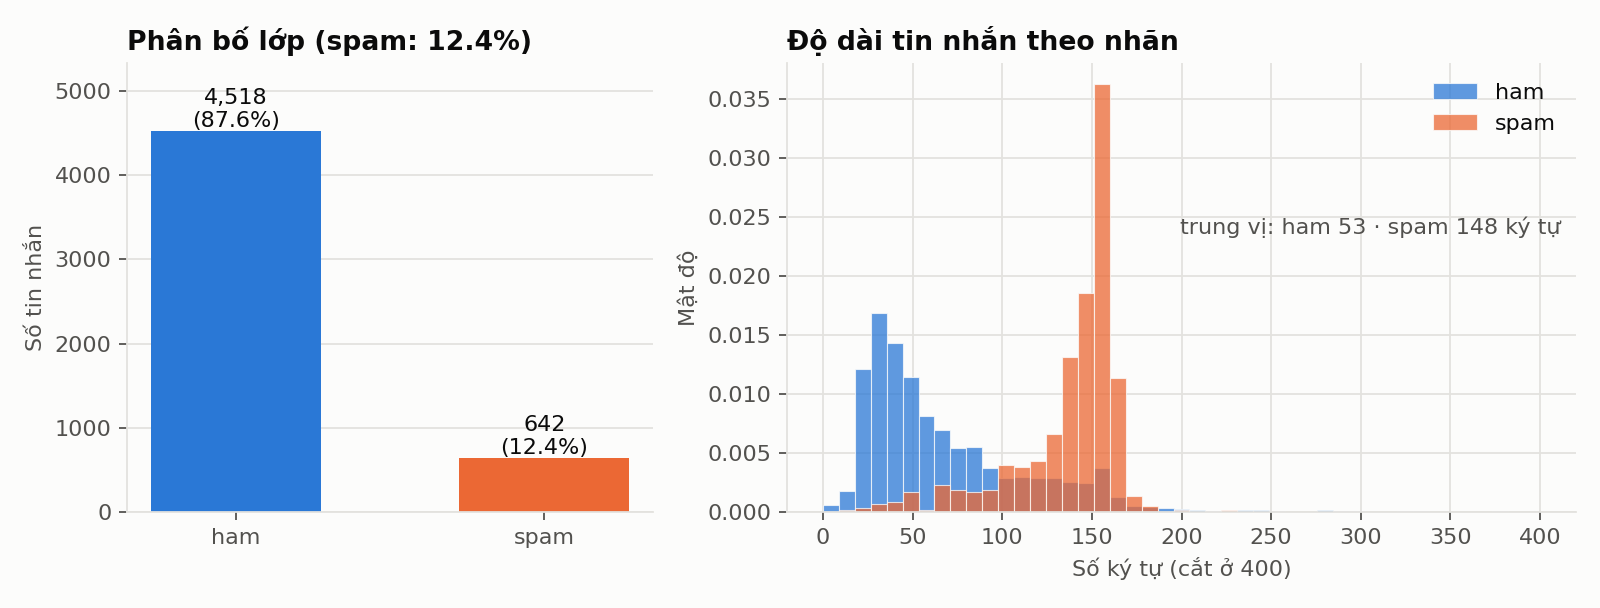
\includegraphics[width=\textwidth]{images/viz_1_class_balance.png}
    \caption{Phân bố lớp (trái) và phân bố độ dài tin nhắn theo nhãn (phải)}
    \label{fig:eda-balance}
    \Nguon{Nhóm xây dựng từ dữ liệu SMS Spam Collection (đã loại trùng)}
\end{figure}

\subsection{Độ dài tin nhắn}

Spam dài hơn rõ rệt: độ dài trung vị là \textbf{148 ký tự} (25 từ) so với \textbf{53 ký tự} (11 từ) của ham; trung bình lần lượt là 137,4 và 70,9 ký tự. Phân bố độ dài của spam tập trung thành một đỉnh nhọn quanh 150--160 ký tự, sát giới hạn 160 ký tự của một SMS, phản ánh việc spam thường được soạn sẵn để dùng trọn một tin nhắn (Hình~\ref{fig:eda-balance}, bên phải). Đây là đặc trưng mạnh, nhưng chồng lấn đáng kể ở vùng 100--150 ký tự nên không thể dùng riêng lẻ.

\subsection{Các đặc điểm cấu trúc gợi ý}

Nhóm khảo sát tỉ lệ tin chứa từng đặc điểm theo nhãn (Bảng~\ref{tab:dac-diem}).

\begin{table}[H]
\centering
\caption{Tỉ lệ tin nhắn chứa các đặc điểm cấu trúc theo nhãn}
\label{tab:dac-diem}
\begin{tabular}{|p{6.4cm}|c|c|}
\hline
\textbf{Đặc điểm} & \textbf{Spam (\%)} & \textbf{Ham (\%)} \\
\hline
Có ít nhất một chữ số & 93,9 & 15,8 \\
\hline
Có chuỗi từ 5 chữ số trở lên (số điện thoại, đầu số) & 76,5 & 0,1 \\
\hline
Có tên miền hoặc URL & 17,4 & 0,2 \\
\hline
Có ký hiệu tiền tệ (\textit{£}, \$, \texteuro) & 33,3 & 0,4 \\
\hline
Có từ viết hoa toàn bộ (từ 3 chữ cái trở lên) & 69,2 & 6,4 \\
\hline
Có dấu \texttt{!} & 47,0 & 11,7 \\
\hline
\end{tabular}
\Nguon{Nhóm tính trên 5\,160 tin sau khi loại trùng}
\end{table}

Bảng~\ref{tab:dac-diem} cho thấy chuỗi số dài, ký hiệu tiền và URL là tín hiệu gần như \textit{độc quyền} của spam. Đây là cơ sở thực nghiệm cho quyết định \textbf{không xóa số, tiền, URL} trong tiền xử lý mà thay bằng token đại diện (Mục~\ref{sec:tien-xu-ly}).

\subsection{Từ phổ biến theo lớp và giả thuyết ban đầu}

\begin{figure}[H]
    \centering
    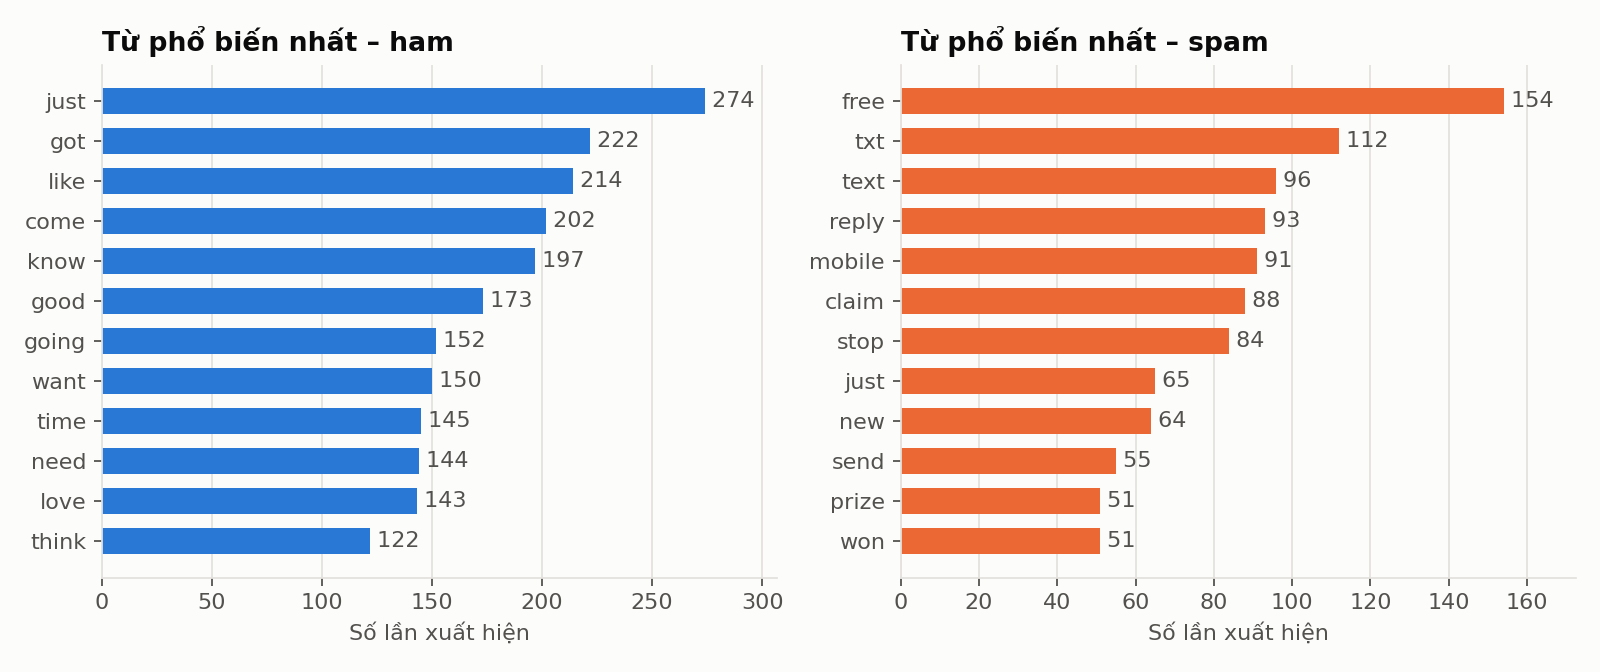
\includegraphics[width=\textwidth]{images/viz_2_top_words.png}
    \caption{Các từ phổ biến nhất của lớp ham (trái) và spam (phải), đã bỏ từ dừng}
    \label{fig:eda-topwords}
    \Nguon{Nhóm xây dựng từ dữ liệu SMS Spam Collection (đã loại trùng)}
\end{figure}

Từ phổ biến của ham là các từ hội thoại đời thường (\textit{just, got, like, come, know, love}), còn của spam là các từ kêu gọi hành động và khuyến mãi (\textit{free, txt, text, reply, mobile, claim, stop, prize, won}). Từ đó nhóm rút ra các \textbf{giả thuyết} để kiểm chứng ở các chương sau:

\begin{enumerate}[label=\textbf{H\arabic*.}]
    \item Từ khóa khuyến mãi và lời kêu gọi hành động là tín hiệu mạnh; một mô hình dựa trên đếm từ đã đạt chất lượng cao.
    \item Các cụm hai từ (\textit{to claim}, \textit{have won}) mang thêm thông tin so với từ đơn.
    \item Giữ lại tín hiệu số/tiền/URL (dưới dạng token) có lợi hơn xóa chúng; còn bỏ từ dừng có thể gây hại vì các từ như \textit{call}, \textit{to}, \textit{your} cũng mang tín hiệu.
\end{enumerate}

\section{Tiền xử lý văn bản}
\label{sec:tien-xu-ly}

\subsection{Nguyên tắc thiết kế}

Với bài toán spam, nhiều bước ``làm sạch'' kinh điển lại \textit{xóa mất tín hiệu}. Nhóm áp dụng ba nguyên tắc:

\begin{enumerate}[label=(\arabic*)]
    \item \textbf{Không xóa, mà thay thế bằng token.} URL, số tiền và số được thay bằng \texttt{urltoken}, \texttt{moneytoken}, \texttt{numtoken}. Các token này chỉ gồm chữ cái để không bị bước bỏ dấu câu/số xóa nhầm. Nhờ đó mô hình học được \textit{``có xuất hiện một URL/số tiền/số''} thay vì phải học từng giá trị cụ thể (mỗi số điện thoại hầu như chỉ xuất hiện một lần).
    \item \textbf{Mỗi bước phải bật/tắt độc lập} để làm thí nghiệm đối chứng (ablation) và có bằng chứng định lượng.
    \item \textbf{Bước tiền xử lý không học gì từ dữ liệu} (phương thức \texttt{fit} của \texttt{TextCleaner} không làm gì), vì vậy bản thân nó không thể gây rò rỉ.
\end{enumerate}

\subsection{Các bước và thứ tự áp dụng}

\begin{table}[H]
\centering
\caption{Các tùy chọn của bộ làm sạch văn bản \texttt{TextCleaner}}
\label{tab:cleaner}
\begin{tabular}{|c|p{3.6cm}|p{8.6cm}|}
\hline
\textbf{STT} & \textbf{Tùy chọn} & \textbf{Hành vi và lý do} \\
\hline
1 & \texttt{lowercase} (luôn bật) & Đưa về chữ thường để \textit{FREE} và \textit{free} là một. \\
\hline
2 & \texttt{replace\_url} & Thay URL/tên miền bằng \texttt{urltoken}; dấu câu cuối câu được giữ lại bên ngoài token. \\
\hline
3 & \texttt{replace\_money} & Thay mẫu tiền tệ (\textit{£900}, \textit{\$5}, \textit{50p}, \textit{10 pounds}) bằng \texttt{moneytoken}. Chạy trước bước số vì số tiền chứa chữ số. \\
\hline
4 & \texttt{replace\_number} & Thay mọi chuỗi chữ số còn lại bằng \texttt{numtoken}. \\
\hline
5 & \texttt{remove\_punct} & Thay ký tự không phải chữ/số/khoảng trắng bằng khoảng trắng. \\
\hline
6 & \texttt{remove\_stopwords} & Bỏ từ dừng tiếng Anh (danh sách của scikit-learn); mặc định tắt. \\
\hline
\end{tabular}
\Nguon{Nhóm xây dựng; mã nguồn \texttt{spam\_filter/preprocessing.py}}
\end{table}

Thứ tự (URL $\to$ tiền $\to$ số $\to$ dấu câu) có ý nghĩa: nếu bỏ dấu câu trước, \texttt{www.cashbin.co.uk} sẽ bị cắt thành năm mảnh vô nghĩa, còn nếu thay số trước thì \textit{£900} chỉ còn \textit{£numtoken}.

\subsection{Ví dụ minh họa}

Áp dụng lên tin nhắn mẫu \textit{``WINNER!! As a valued network customer you have been selected to receivea £900 prize reward! To claim call 09061701461. Claim code KL341. Valid 12 hours only.''}:

\begin{table}[H]
\centering
\caption{Đầu ra của bộ làm sạch với các cấu hình khác nhau}
\label{tab:vi-du-lam-sach}
\begin{tabular}{|p{3.4cm}|p{10.8cm}|}
\hline
\textbf{Cấu hình} & \textbf{Kết quả} \\
\hline
Chỉ chữ thường (E0--E4) & \textit{winner!! as a valued network customer you have been selected to receivea £900 prize reward! to claim call 09061701461. claim code kl341. valid 12 hours only.} \\
\hline
Token hóa URL/tiền/số và bỏ dấu câu (E5) & \textit{winner as a valued network customer you have been selected to receivea moneytoken prize reward to claim call numtoken claim code kl numtoken valid numtoken hours only} \\
\hline
Bỏ dấu câu và bỏ stopword (E6) & \textit{winner valued network customer selected receivea 900 prize reward claim 09061701461 claim code kl341 valid 12 hours} \\
\hline
\end{tabular}
\Nguon{Nhóm chạy trực tiếp lớp \texttt{TextCleaner}}
\end{table}

Có thể thấy cấu hình E5 biến số điện thoại 11 chữ số và mã \textit{KL341} (vốn là các token duy nhất, vô dụng khi mô hình gặp tin mới) thành các token chung \texttt{numtoken}, trong khi cấu hình E6 giữ nguyên chúng nhưng làm mất các từ như \textit{to}, \textit{you}, \textit{have}.

\section{Biểu diễn đặc trưng}

Hai phương án biểu diễn được cài đặt bằng \texttt{CountVectorizer} (BoW) và \texttt{TfidfVectorizer} (TF-IDF) của scikit-learn, với các tham số được thay đổi có kiểm soát (Bảng~\ref{tab:vectorizer}).

\begin{table}[H]
\centering
\caption{Các cấu hình vector hóa được khảo sát}
\label{tab:vectorizer}
\begin{tabular}{|p{3.6cm}|p{4.6cm}|p{5.8cm}|}
\hline
\textbf{Tham số} & \textbf{Giá trị khảo sát} & \textbf{Mục đích} \\
\hline
Loại biểu diễn & BoW, TF-IDF & Đếm thô so với có trọng số độ hiếm \\
\hline
\texttt{ngram\_range} & $(1,1)$, $(1,2)$ & Đo lợi ích của cụm hai từ \\
\hline
\texttt{min\_df} & 1, 2, 5 & Cân bằng giữa nhiễu và mất từ hiếm \\
\hline
\texttt{max\_df} & 0,9; 1,0 & Loại từ xuất hiện quá phổ biến \\
\hline
\end{tabular}
\Nguon{Nhóm xây dựng}
\end{table}

Từ vựng được xây dựng \textbf{chỉ từ tập huấn luyện}. Với cấu hình tốt nhất (TF-IDF bigram, \texttt{min\_df}=2, có token hóa), từ vựng gồm 9\,952 n-gram. Vector TF-IDF được chuẩn hóa $L_2$ theo mặc định.

\chapter{THIẾT KẾ PIPELINE VÀ THIẾT LẬP THÍ NGHIỆM}

\section{Kiến trúc tổng thể}

Toàn bộ quy trình được cài đặt thành thư viện Python \texttt{spam\_filter} và dùng chung cho dòng lệnh, notebook và ứng dụng web. Luồng xử lý được thể hiện ở Sơ đồ~\ref{fig:so-do-pipeline}.

\begin{sodo}[H]
    \centering
    \resizebox{\textwidth}{!}{%
    \begin{tikzpicture}[
        node distance=0.55cm and 0.7cm,
        box/.style={draw, rounded corners=2pt, align=center, minimum height=1.05cm, minimum width=2.3cm, font=\small, fill=gray!8},
        data/.style={box, fill=blue!8},
        keep/.style={box, fill=green!10},
        arr/.style={-{Latex[length=2mm]}, thick}
    ]
        \node[data] (raw) {Dữ liệu thô\\5\,574 tin};
        \node[box, right=of raw] (dedup) {Loại trùng\\$\to$ 5\,160 tin};
        \node[box, right=of dedup] (split) {Chia 80/20\\phân tầng, seed 42};
        \node[keep, below=1.1cm of split, xshift=-2.2cm] (test) {Tập kiểm tra\\1\,032 tin};
        \node[box, below=1.1cm of split, xshift=2.2cm] (train) {Tập huấn luyện\\4\,128 tin};
        \node[box, right=1.6cm of train, minimum width=2.8cm] (pipe) {\textbf{Pipeline}\\Làm sạch $\to$ Vector hóa\\$\to$ Mô hình};
        \node[box, below=0.9cm of pipe] (cv) {CV 5-fold\\(F1 lớp spam)};
        \node[box, below=0.9cm of train] (select) {Chọn mô hình\\theo CV F1};
        \node[keep, below=0.9cm of test] (eval) {Đánh giá cuối\\Acc/P/R/F1/AUC};
        \node[box, left=0.7cm of eval] (err) {Phân tích lỗi\\và kiểm tra rò rỉ};

        \draw[arr] (raw) -- (dedup);
        \draw[arr] (dedup) -- (split);
        \draw[arr] (split) -- (test);
        \draw[arr] (split) -- (train);
        \draw[arr] (train) -- (pipe);
        \draw[arr] (pipe) -- (cv);
        \draw[arr] (cv) -- (select);
        \draw[arr] (select) -| (eval);
        \draw[arr, dashed] (test) -- (eval);
        \draw[arr] (eval) -- (err);
    \end{tikzpicture}}
    \SodoCaption{Luồng xử lý của pipeline phân loại spam (tập kiểm tra, màu xanh lá, chỉ dùng ở bước đánh giá cuối)}{Nhóm xây dựng}
    \label{fig:so-do-pipeline}
\end{sodo}

\textbf{Điểm then chốt về chống rò rỉ.} Ba bước ``làm sạch, vector hóa, mô hình'' được ghép thành một đối tượng \texttt{Pipeline}. Khi gọi \texttt{fit} trên tập huấn luyện (hoặc trên $K-1$ fold trong CV), từ vựng và trọng số IDF chỉ được tính từ phần dữ liệu đó; khi dự đoán trên dữ liệu mới, vector hóa chỉ \textit{áp dụng} (\texttt{transform}) mà không học lại. Nếu vectorizer bị \texttt{fit} trên toàn bộ dữ liệu trước khi chia, từ vựng và IDF của tập test sẽ ``lọt'' vào mô hình, và kết quả sẽ lạc quan hơn thực tế.

\section{Tổ chức mã nguồn}

\begin{table}[H]
\centering
\caption{Các mô-đun của thư viện \texttt{spam\_filter}}
\label{tab:modules}
\begin{tabular}{|p{3.6cm}|p{10.4cm}|}
\hline
\textbf{Mô-đun} & \textbf{Trách nhiệm} \\
\hline
\texttt{config.py} & Đường dẫn, tên cột, \texttt{random\_state}, tỉ lệ chia, số fold; \textit{nơi duy nhất cần sửa khi đổi dữ liệu}. \\
\hline
\texttt{data.py} & Đọc dữ liệu, chuẩn hóa nhãn, loại trùng, chia train/test có phân tầng. \\
\hline
\texttt{preprocessing.py} & \texttt{TextCleaner}: các bước làm sạch bật/tắt được. \\
\hline
\texttt{features.py} & Tạo \texttt{CountVectorizer} hoặc \texttt{TfidfVectorizer}. \\
\hline
\texttt{models.py} & Khai báo Multinomial NB, K-NN (cosine), Decision Tree. \\
\hline
\texttt{pipeline.py} & \texttt{ExperimentSpec} và \texttt{build\_pipeline}. \\
\hline
\texttt{experiments.py} & Danh sách thí nghiệm E0--E6; thêm thí nghiệm bằng cách thêm một dòng. \\
\hline
\texttt{runner.py} & Chạy danh sách thí nghiệm và xuất bảng kết quả. \\
\hline
\texttt{evaluation.py} & Các thước đo, CV phân tầng, ma trận nhầm lẫn. \\
\hline
\texttt{error\_analysis.py} & Liệt kê FP/FN; từ đặc trưng spam/ham của Naive Bayes. \\
\hline
\texttt{sanity.py} & Kiểm tra rò rỉ, học thuộc, baseline đơn giản; đường cong học. \\
\hline
\texttt{eda.py}, \texttt{viz.py} & Thống kê và biểu đồ khám phá/báo cáo. \\
\hline
\texttt{cli.py} & Các lệnh \texttt{eda}, \texttt{run}, \texttt{viz}, \texttt{check}, \texttt{predict}. \\
\hline
\end{tabular}
\Nguon{Nhóm xây dựng}
\end{table}

Thiết kế dựa trên cấu hình khai báo: mỗi thí nghiệm là một đối tượng \texttt{ExperimentSpec} (tên, mô hình, tham số mô hình, tham số làm sạch, tham số vector hóa). Cách này tách \textit{``chạy cái gì''} khỏi \textit{``chạy như thế nào''}, khiến việc ghi log tham số và mở rộng thí nghiệm trở nên tầm thường và ít lỗi.

\section{Thiết lập thực nghiệm}

\subsection{Chia dữ liệu và hạt giống ngẫu nhiên}

\begin{itemize}
    \item Chia \textbf{80\% huấn luyện / 20\% kiểm tra}, \texttt{stratify} theo nhãn, \texttt{random\_state}=42.
    \item Loại bản trùng \textit{trước} khi chia để không có tin giống hệt nhau ở hai tập (kiểm chứng ở Mục~\ref{sec:sanity}, kiểm tra A1).
    \item Kiểm định chéo phân tầng 5 fold, có xáo trộn, \texttt{random\_state}=42, \textbf{chỉ trên tập huấn luyện}.
    \item Tiêu chí chọn mô hình: \textbf{F1 của lớp spam trung bình qua CV}, tuyệt đối không dùng tập kiểm tra để chọn.
\end{itemize}

\subsection{Danh sách thí nghiệm}

Bảng~\ref{tab:thi-nghiem} là nhật ký thí nghiệm gồm một baseline, các biến thể biểu diễn/mô hình và hai thí nghiệm đối chứng về tiền xử lý.

\begin{table}[H]
\centering
\caption{Danh sách thí nghiệm và tham số (nhật ký thí nghiệm)}
\label{tab:thi-nghiem}
\small
\begin{tabular}{|c|p{3.2cm}|p{2.9cm}|p{3.3cm}|p{2.2cm}|}
\hline
\textbf{ID} & \textbf{Làm sạch} & \textbf{Vector hóa} & \textbf{Mô hình} & \textbf{Vai trò} \\
\hline
E0 & Chữ thường & BoW, unigram & MultinomialNB, $\alpha=1$ (mặc định) & \textbf{Baseline} \\
\hline
E1 & Chữ thường & TF-IDF, unigram & MultinomialNB, $\alpha=0{,}5$ & Đổi biểu diễn \\
\hline
E2 & Chữ thường & TF-IDF, $(1,2)$-gram, \texttt{min\_df}=2 & MultinomialNB, $\alpha=0{,}1$ & Thêm bigram, chỉnh $\alpha$ \\
\hline
E3 & Chữ thường & TF-IDF, unigram, \texttt{min\_df}=2 & K-NN, $k=5$, cosine & Thuật toán 2 \\
\hline
E4 & Chữ thường & TF-IDF, unigram, \texttt{min\_df}=2 & Decision Tree, \texttt{max\_depth}=20, \texttt{min\_samples\_leaf}=2 & Thuật toán 3 \\
\hline
E5 & Token hóa URL/tiền/số, bỏ dấu câu & Như E2 & MultinomialNB, $\alpha=0{,}1$ & Ablation (token hóa) \\
\hline
E6 & Bỏ dấu câu, bỏ stopword & Như E2 & MultinomialNB, $\alpha=0{,}1$ & Ablation (stopword) \\
\hline
\end{tabular}
\Nguon{Nhóm xây dựng; mã nguồn \texttt{spam\_filter/experiments.py}}
\end{table}

\textbf{Lưu ý về thiết kế thí nghiệm.} E5 và E6 thay đổi \textit{đúng một khía cạnh} so với E2 (cách làm sạch), cho phép quy kết chênh lệch kết quả cho khía cạnh đó. Ngược lại E0$\to$E1$\to$E2 thay đổi đồng thời biểu diễn và tham số $\alpha$, nên để tách tác động riêng lẻ nhóm bổ sung phân tích độ nhạy theo từng tham số ở Mục~\ref{sec:nhay-tham-so}.

\subsection{Môi trường tái lập}

\begin{table}[H]
\centering
\caption{Môi trường thực nghiệm}
\label{tab:moi-truong}
\begin{tabular}{|p{5cm}|p{9cm}|}
\hline
\textbf{Thành phần} & \textbf{Phiên bản} \\
\hline
Python & 3.14.6 \\
\hline
Thư viện chính & scikit-learn \cite{scikit-learn}, NumPy \cite{numpy2020}, pandas \cite{pandas2010}, matplotlib \cite{matplotlib2007} \\
\hline
scikit-learn & 1.9.0 \\
\hline
NumPy / pandas & 2.4.1 / 3.1.0 \\
\hline
Tệp \texttt{requirements.txt} & Chỉ đặt phiên bản \textit{tối thiểu} (không khóa cứng) \\
\hline
\end{tabular}
\Nguon{Nhóm ghi nhận khi chạy lại toàn bộ thí nghiệm}
\end{table}

Do \texttt{requirements.txt} không khóa phiên bản, kết quả có thể lệch nhẹ ở chữ số thập phân thứ ba khi dùng phiên bản thư viện khác. Các lệnh tái lập đầy đủ nằm ở Phụ lục~1.

\subsection{Kiểm thử tự động}

Mã nguồn đi kèm \textbf{41 bài kiểm thử} (pytest) trong năm tệp: \texttt{test\_data.py} (đọc dữ liệu, ánh xạ nhãn, loại trùng, chia phân tầng, không trùng văn bản giữa train và test, tái lập theo hạt giống), \texttt{test\_pipeline.py} (hành vi của \texttt{TextCleaner} với URL, tiền, số, stopword và việc mọi thí nghiệm đều huấn luyện và dự đoán được), \texttt{test\_evaluation.py} (đúng các thước đo và chiều của ma trận nhầm lẫn), \texttt{test\_serialization.py} (lưu rồi tải mô hình cho dự đoán giống hệt) và \texttt{test\_reporting.py} (bảng kết quả và biểu đồ báo cáo). Toàn bộ 41 kiểm thử đều đạt tại thời điểm viết báo cáo.

\chapter{KẾT QUẢ THỰC NGHIỆM VÀ SO SÁNH}

Chương này trình bày kết quả của bảy thí nghiệm E0--E6. Quy ước đọc số liệu: cột \textbf{CV F1} là F1 của lớp spam trung bình qua kiểm định chéo 5 fold \textit{chỉ trên tập huấn luyện} và là căn cứ chọn mô hình; các cột \textbf{Test} được tính trên tập kiểm tra giữ riêng (1\,032 tin, trong đó 128 spam) và chỉ dùng để báo cáo.

\section{Kết quả tổng hợp}

\begin{table}[H]
\centering
\caption{Kết quả của các thí nghiệm trên tập kiểm tra ($\text{spam}$ là lớp dương)}
\label{tab:ket-qua}
\small
\begin{tabular}{|c|c|c|c|c|c|c|c|}
\hline
\textbf{ID} & \textbf{CV F1} & \textbf{Acc.} & \textbf{Prec.} & \textbf{Recall} & \textbf{F1} & \textbf{AUC} & \textbf{TN/FP/FN/TP} \\
\hline
E0 (baseline) & 0,9385 & 0,9826 & 0,9508 & 0,9062 & 0,9280 & 0,9790 & 898/6/12/116 \\
\hline
E1 & 0,8512 & 0,9719 & 0,9901 & 0,7812 & 0,8734 & 0,9832 & 903/1/28/100 \\
\hline
E2 & 0,9365 & 0,9845 & 0,9746 & 0,8984 & 0,9350 & 0,9882 & 901/3/13/115 \\
\hline
E3 (K-NN) & 0,8935 & 0,9758 & 0,9640 & 0,8359 & 0,8954 & 0,9685 & 900/4/21/107 \\
\hline
E4 (Cây) & 0,8086 & 0,9700 & 0,9450 & 0,8047 & 0,8692 & 0,8954 & 898/6/25/103 \\
\hline
\textbf{E5} & \textbf{0,9425} & \textbf{0,9864} & 0,9750 & \textbf{0,9141} & \textbf{0,9435} & 0,9905 & 901/3/11/117 \\
\hline
E6 & 0,9283 & 0,9845 & 0,9746 & 0,8984 & 0,9350 & 0,9920 & 901/3/13/115 \\
\hline
\end{tabular}
\Nguon{Nhóm tổng hợp từ tệp \texttt{outputs/results/metrics.csv}}
\end{table}

Theo tiêu chí đã đặt trước (CV F1), \textbf{E5 là cấu hình tốt nhất}: Accuracy 98,64\%, Precision 97,50\%, Recall 91,41\%, F1 94,35\%, ROC-AUC 0,9905. Trên 1\,032 tin kiểm tra mô hình chặn nhầm 3 tin hợp lệ và bỏ lọt 11 tin spam.

Ma trận nhầm lẫn chi tiết của E5 nằm ở Phụ lục 2 (Hình~\ref{fig:cm-e5}).

\begin{figure}[H]
    \centering
    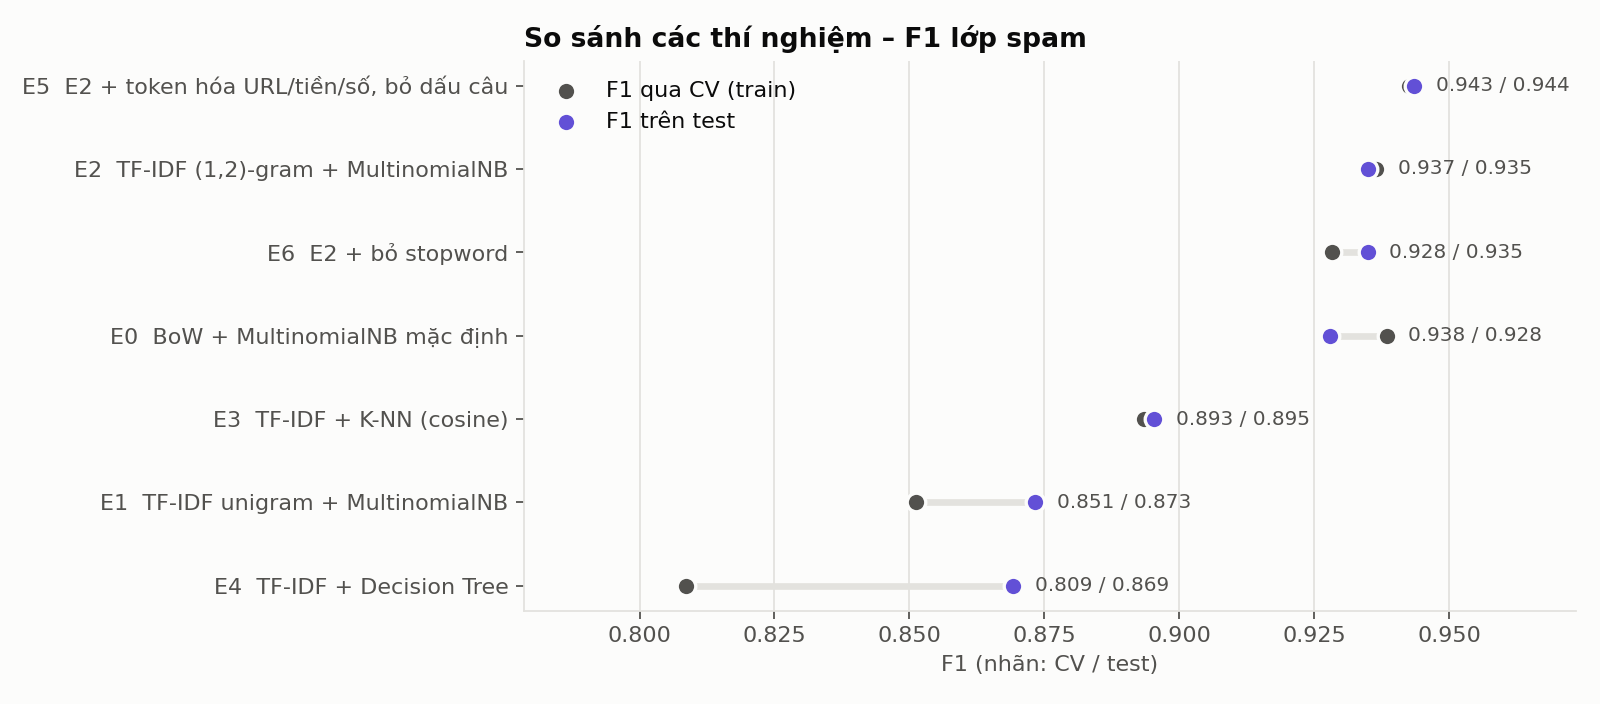
\includegraphics[width=\textwidth]{images/viz_3_model_comparison.png}
    \caption{So sánh F1 của lớp spam giữa kiểm định chéo (chấm đen) và tập kiểm tra (chấm tím)}
    \label{fig:so-sanh-mo-hinh}
    \Nguon{Nhóm xây dựng từ kết quả thí nghiệm}
\end{figure}

\begin{figure}[H]
    \centering
    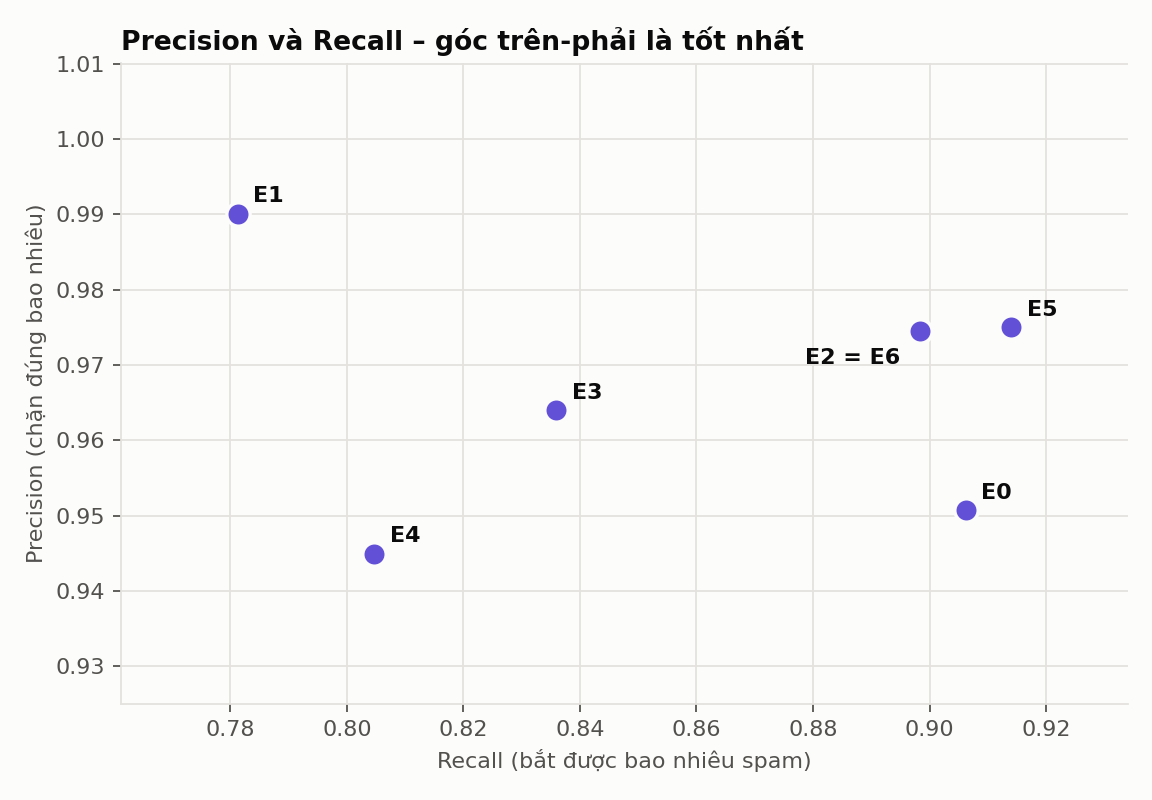
\includegraphics[width=0.78\textwidth]{images/viz_4_precision_recall.png}
    \caption{Precision và Recall của các thí nghiệm trên tập kiểm tra}
    \label{fig:precision-recall}
    \Nguon{Nhóm xây dựng từ kết quả thí nghiệm}
\end{figure}

\subsection{Nhận xét theo từng nhóm}

\textbf{(1) Họ Naive Bayes vượt trội K-NN và Cây quyết định.} Trong ba thuật toán, các biến thể Naive Bayes tốt (E0, E2, E5, E6) cho F1 kiểm tra 0,928--0,944, trong khi K-NN (E3) đạt 0,895 và Decision Tree (E4) chỉ 0,869 với Recall 80,5\%. Qua 10 lần chia ngẫu nhiên (Mục~\ref{sec:on-dinh}) khoảng cách này lặp lại ở \textbf{mọi} lần chia: E0 hơn E3 ở 10/10 lần với chênh lệch trung bình 0,037. Giải thích phù hợp với lý thuyết: K-NN chịu lời nguyền số chiều trên không gian từ vựng hàng nghìn chiều, còn cây đơn thường chỉ dựa vào một số ít từ khóa nên bỏ lọt các spam ``viết khéo''.

\textbf{(2) Accuracy gần như vô nghĩa để phân biệt mô hình.} Mọi thí nghiệm đều có Accuracy từ 97,0\% đến 98,6\%, trong khi mô hình luôn đoán ``ham'' đã đạt 87,6\%. Khoảng cách giữa E5 (98,64\%) và E4 (97,00\%) trông nhỏ nhưng tương ứng với số spam bỏ lọt tăng từ 11 lên 25, tức Recall giảm từ 91,4\% xuống 80,5\%. Đây là lý do nhóm dùng F1 của lớp spam.

\textbf{(3) Đánh đổi Precision--Recall của E1.} E1 có Precision cao nhất (99,01\%, chỉ 1 tin ham bị chặn nhầm) nhưng Recall thấp nhất trong nhóm NB (78,12\%, bỏ lọt 28 spam). Mô hình quá thận trọng. Nguyên nhân được truy vết ở Mục~\ref{sec:nhay-tham-so}: tham số làm mượt $\alpha=0{,}5$ quá lớn so với thang giá trị của TF-IDF.

\textbf{(4) Mức độ quá khớp.} Hình~\ref{fig:overfit} cho thấy khoảng cách F1 giữa huấn luyện và kiểm tra nằm trong khoảng $+0{,}037$ đến $+0{,}074$ với mọi mô hình, không có dấu hiệu học thuộc nghiêm trọng. Với E5, F1 huấn luyện là 0,983 và kiểm tra là 0,944.

\begin{figure}[H]
    \centering
    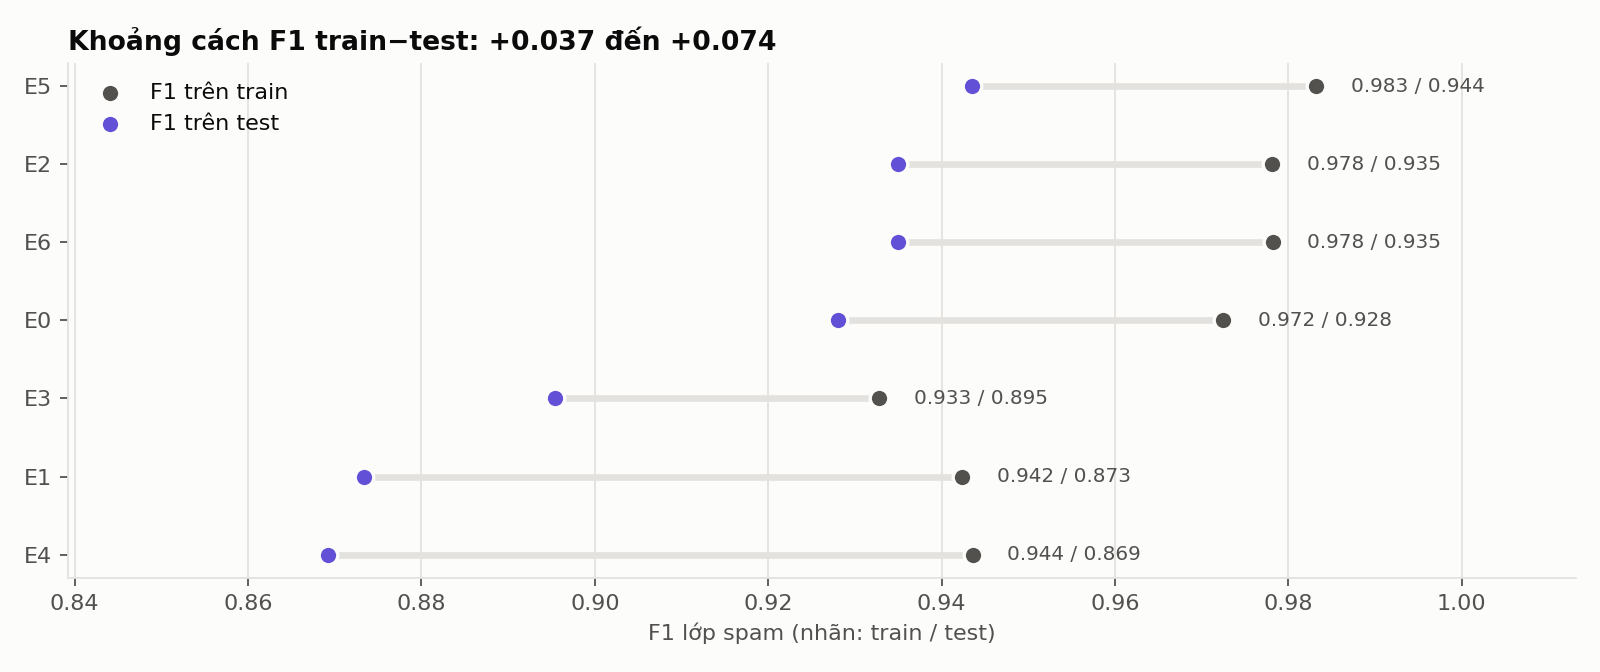
\includegraphics[width=0.95\textwidth]{images/viz_6_overfitting_check.png}
    \caption{Khoảng cách F1 giữa tập huấn luyện và tập kiểm tra}
    \label{fig:overfit}
    \Nguon{Nhóm xây dựng từ kết quả thí nghiệm}
\end{figure}

\section{Độ nhạy theo tham số và thí nghiệm đối chứng}
\label{sec:nhay-tham-so}

Do các thí nghiệm E0--E6 thay đổi nhiều yếu tố cùng lúc, nhóm bổ sung một chuỗi thí nghiệm \textit{thay đổi từng yếu tố một}, đo bằng CV F1 trên tập huấn luyện (không chạm vào tập kiểm tra). Cấu hình nền là cấu hình của E5 (token hóa, TF-IDF $(1,2)$-gram, \texttt{min\_df}=2, $\alpha=0{,}1$), trừ khi nêu khác.

\begin{table}[H]
\centering
\caption{Độ nhạy của CV F1 theo từng yếu tố (cấu hình nền E5; $\alpha$ cố định 0,1 trừ dòng khảo sát $\alpha$)}
\label{tab:nhay}
\begin{tabular}{|p{4.4cm}|p{5.2cm}|c|}
\hline
\textbf{Yếu tố} & \textbf{Giá trị} & \textbf{CV F1} \\
\hline
\multirow{4}{4.4cm}{Biểu diễn và n-gram (\texttt{min\_df}=2)}
 & BoW, unigram & 0,9469 \\
\cline{2-3}
 & BoW, $(1,2)$-gram & 0,9405 \\
\cline{2-3}
 & TF-IDF, unigram & 0,9439 \\
\cline{2-3}
 & TF-IDF, $(1,2)$-gram & 0,9425 \\
\hline
\multirow{3}{4.4cm}{\texttt{min\_df} (TF-IDF, bigram)}
 & 1 & 0,9472 \\
\cline{2-3}
 & 2 & 0,9425 \\
\cline{2-3}
 & 5 & 0,9366 \\
\hline
\multirow{2}{4.4cm}{\texttt{max\_df}}
 & 0,9 & 0,9425 \\
\cline{2-3}
 & 1,0 & 0,9425 \\
\hline
\multirow{5}{4.4cm}{Làm mượt $\alpha$ (TF-IDF, bigram)}
 & 0,01 & 0,9436 \\
\cline{2-3}
 & 0,05 & 0,9427 \\
\cline{2-3}
 & 0,1 & 0,9425 \\
\cline{2-3}
 & 0,5 & 0,9123 \\
\cline{2-3}
 & 1,0 & 0,8597 \\
\hline
\end{tabular}
\Nguon{Nhóm thực nghiệm; kết quả trên tập huấn luyện bằng CV phân tầng 5 fold}
\end{table}

\textbf{Phát hiện 1: $\alpha$ là yếu tố có tác động lớn nhất.} CV F1 giữ ổn định ($\approx0{,}943$) với $\alpha\le0{,}1$ rồi sụt mạnh còn 0,9123 ở $\alpha=0{,}5$ và 0,8597 ở $\alpha=1{,}0$. Cơ chế: vector TF-IDF đã chuẩn hóa $L_2$ nên mỗi thành phần $\le1$ và tổng $N_{wc}$ trên một từ nhỏ so với số đếm thô của BoW; một $\alpha$ cố định (ví dụ 1,0) khi đó ``đè bẹp'' tín hiệu của các từ hiếm nhưng quyết định như \textit{prize} hay \textit{claim}, đẩy mô hình về lớp đa số. Đây cũng là lời giải thích hợp lý cho Recall thấp của E1 ($\alpha=0{,}5$) và cho thấy $\alpha$ mặc định của BoW \textit{không chuyển thẳng} sang TF-IDF.

\textbf{Phát hiện 2: không có bằng chứng rằng TF-IDF hay bigram hơn BoW unigram.} Với tham số $\alpha$ phù hợp, bốn tổ hợp biểu diễn/n-gram chỉ chênh nhau trong khoảng 0,9405--0,9469 (biên độ 0,006), nhỏ hơn độ lệch chuẩn khi thay đổi cách chia dữ liệu ($\approx0{,}012$--$0{,}019$, xem Mục~\ref{sec:on-dinh}). Thậm chí BoW unigram có CV F1 nhỉnh nhất. Giả thuyết ban đầu \textbf{H2} (bigram mang thêm thông tin) vì thế \textit{không được kiểm chứng} trên bộ dữ liệu này, một phần vì các từ khóa spam đơn lẻ đã đủ mạnh. Nhóm vẫn giữ cấu hình bigram cho E5 như đã cố định từ trước khi chạy thí nghiệm độ nhạy, và ghi nhận trung thực rằng nó không phải yếu tố tạo khác biệt.

\textbf{Phát hiện 3: \texttt{min\_df}=1 nhỉnh hơn nhẹ, \texttt{max\_df} không có tác dụng.} Giữ cả các n-gram hiếm cho CV F1 cao hơn (0,9472 so với 0,9366 khi \texttt{min\_df}=5), phù hợp với việc nhiều spam chứa các cụm hiếm nhưng đặc trưng. \texttt{max\_df} không thay đổi kết quả vì ít n-gram nào xuất hiện ở trên 90\% văn bản.

\subsection{Thí nghiệm đối chứng về tiền xử lý}

Bảng~\ref{tab:ablation} tách tác động của từng bước làm sạch (cùng vector hóa TF-IDF $(1,2)$-gram, $\alpha=0{,}1$).

\begin{table}[H]
\centering
\caption{Ablation tiền xử lý: CV F1 trên tập huấn luyện}
\label{tab:ablation}
\begin{tabular}{|p{8.6cm}|c|c|}
\hline
\textbf{Cấu hình làm sạch} & \textbf{CV F1} & \textbf{So với E2} \\
\hline
Chỉ chữ thường (E2) & 0,9365 & -- \\
\hline
$+$ bỏ dấu câu & 0,9365 & $0{,}0000$ \\
\hline
$+$ token hóa URL (kèm bỏ dấu câu) & 0,9299 & $-0{,}0066$ \\
\hline
$+$ token hóa tiền (kèm bỏ dấu câu) & 0,9387 & $+0{,}0022$ \\
\hline
$+$ token hóa số (kèm bỏ dấu câu) & 0,9498 & $+0{,}0133$ \\
\hline
Token hóa URL, tiền, số và bỏ dấu câu (E5) & 0,9425 & $+0{,}0060$ \\
\hline
E5 $+$ bỏ stopword & 0,9464 & $+0{,}0099$ \\
\hline
Bỏ dấu câu $+$ bỏ stopword, không token hóa (E6) & 0,9283 & $-0{,}0082$ \\
\hline
\end{tabular}
\Nguon{Nhóm thực nghiệm; E2, E5, E6 trùng với cột CV F1 của Bảng~\ref{tab:ket-qua}}
\end{table}

Các kết luận rút ra, được phát biểu thận trọng:

\begin{itemize}
    \item \textbf{Token hóa số là bước hữu ích nhất} ($+0{,}0133$), nhất quán với EDA (Bảng~\ref{tab:dac-diem}): 76,5\% spam chứa chuỗi từ 5 chữ số trở lên trong khi chỉ 0,1\% ham có. Số điện thoại và đầu số hầu như duy nhất ở mỗi tin, nên nếu không gom về \texttt{numtoken} mô hình không thể khái quát hóa.
    \item \textbf{Token hóa URL đơn lẻ có xu hướng làm giảm} ($-0{,}0066$). Một lý do có thể là bộ nhận diện URL dựa trên biểu thức chính quy sẽ nhận nhầm một số chuỗi như \textit{``co.uk''} trong văn bản thường. Nhóm chưa kiểm chứng riêng nguyên nhân này, vì vậy chỉ nêu như một giả thuyết cần theo dõi.
    \item \textbf{Hiệu quả của việc bỏ stopword không nhất quán về dấu}: làm giảm khi không có token hóa (E6: $-0{,}0082$ so với E2) nhưng làm tăng khi đi cùng token hóa ($+0{,}0039$ so với E5). Với biên độ nhỏ hơn độ biến thiên khi đổi cách chia dữ liệu, kết luận an toàn là \textit{không có bằng chứng bỏ stopword giúp ích}. Điều này phù hợp với giả thuyết \textbf{H3} rằng các từ như \textit{call}, \textit{your} mang tín hiệu, nên không bỏ chúng một cách mặc định.
    \item \textbf{Hiệu ứng cộng gộp}: tổ hợp E5 ($+0{,}0060$) không bằng riêng token hóa số ($+0{,}0133$); các bước tương tác với nhau và không nên chọn theo trực giác ``làm nhiều bước hơn thì tốt hơn''.
\end{itemize}

\textbf{Lưu ý trung thực về lựa chọn E5.} Cấu hình \textit{``chỉ token hóa số''} (CV F1 0,9498) và \textit{BoW unigram} (0,9469) trong các thí nghiệm độ nhạy cho CV F1 cao hơn E5 (0,9425). Cấu hình E5 được định nghĩa và chọn trong bộ thí nghiệm chính E0--E6 \textit{trước khi} chạy phân tích độ nhạy; nhóm không chuyển sang cấu hình khác sau khi nhìn kết quả để tránh tối ưu quá mức trên dữ liệu kiểm định. Ý nghĩa thực tiễn cũng nhỏ: các chênh lệch này nằm trong dải nhiễu của phép đo (Mục~\ref{sec:on-dinh}).

\section{Độ ổn định theo cách chia dữ liệu}
\label{sec:on-dinh}

Tập kiểm tra chỉ có 128 spam nên mỗi tin bị phân loại sai làm F1 thay đổi khoảng 0,4 điểm phần trăm. Để đo độ dao động này, nhóm lặp lại \textit{toàn bộ} quy trình (chia, huấn luyện, kiểm tra) với 10 hạt giống khác nhau $\text{seed}\in\{0,\dots,9\}$.

\begin{table}[H]
\centering
\caption{F1 của lớp spam trên tập kiểm tra qua 10 lần chia ngẫu nhiên}
\label{tab:on-dinh}
\begin{tabular}{|c|c|c|c|c|}
\hline
\textbf{ID} & \textbf{Trung bình} & \textbf{Độ lệch chuẩn} & \textbf{Nhỏ nhất} & \textbf{Lớn nhất} \\
\hline
E5 & 0,9484 & 0,0140 & 0,9256 & 0,9721 \\
\hline
E2 & 0,9428 & 0,0187 & 0,9076 & 0,9636 \\
\hline
E0 & 0,9411 & 0,0124 & 0,9180 & 0,9603 \\
\hline
E6 & 0,9357 & 0,0125 & 0,9076 & 0,9558 \\
\hline
E3 & 0,9040 & 0,0120 & 0,8841 & 0,9218 \\
\hline
E1 & 0,8657 & 0,0156 & 0,8364 & 0,8821 \\
\hline
E4 & 0,8382 & 0,0236 & 0,7951 & 0,8714 \\
\hline
\end{tabular}
\Nguon{Nhóm thực nghiệm (lệnh \texttt{python -m spam\_filter viz --stability})}
\end{table}

\begin{figure}[H]
    \centering
    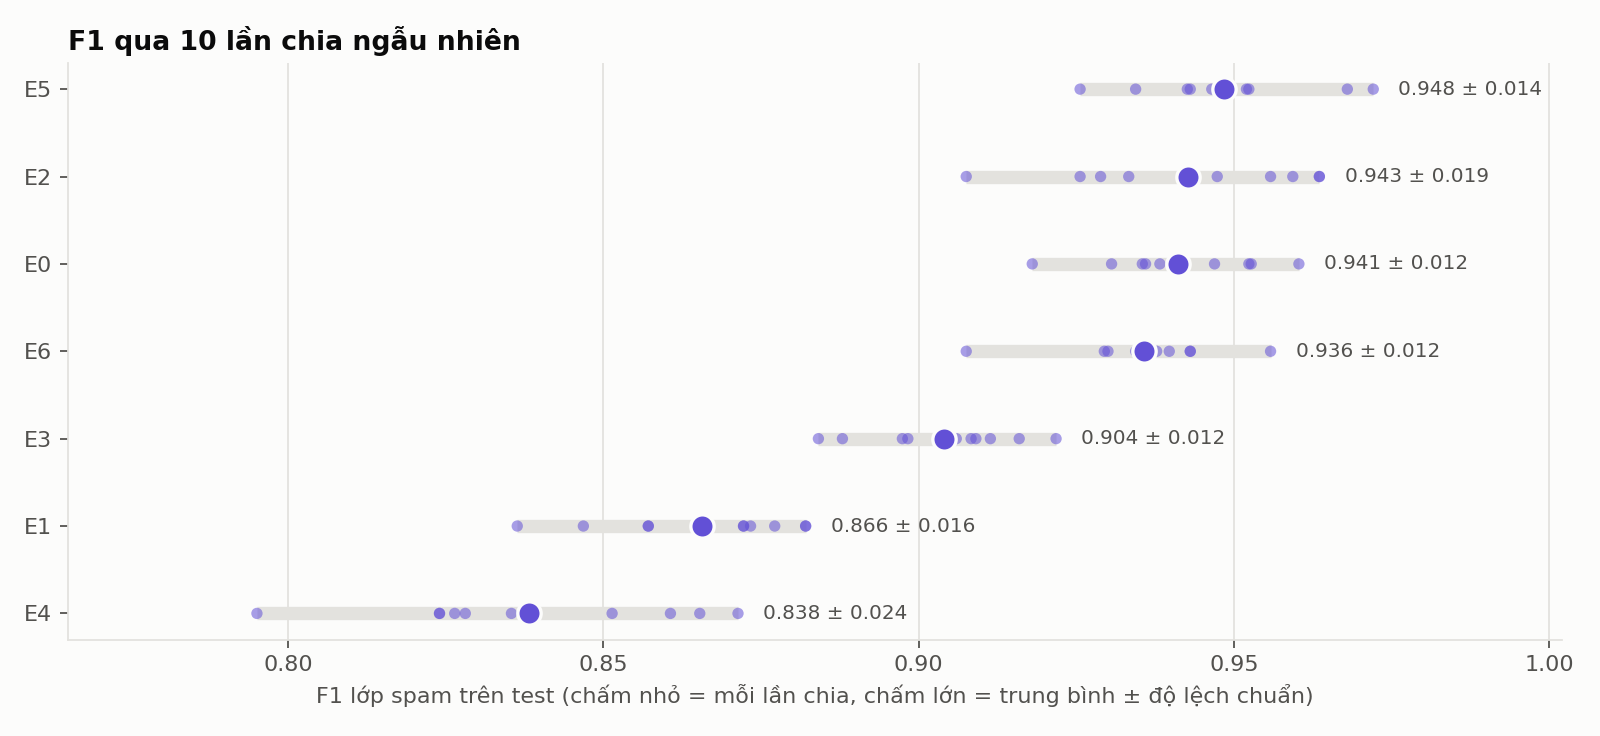
\includegraphics[width=0.95\textwidth]{images/viz_8_f1_stability.png}
    \caption{Phân bố F1 trên tập kiểm tra qua 10 lần chia ngẫu nhiên}
    \label{fig:on-dinh}
    \Nguon{Nhóm xây dựng từ kết quả thí nghiệm}
\end{figure}

Có hai điều rút ra. Thứ nhất, độ lệch chuẩn của F1 là 0,012--0,024, \textbf{lớn hơn khoảng cách giữa E5, E2, E0 và E6} (biên độ trung bình 0,013). Nói cách khác \textit{một lần chia duy nhất không đủ để xếp hạng} nhóm NB. So sánh theo cặp trên cùng cách chia cho thấy E5 hơn E0 trung bình $+0{,}0073\pm0{,}0080$ (thắng 7 trên 10 lần, hòa 1) và hơn E2 trung bình $+0{,}0056\pm0{,}0104$ (thắng 5, hòa 3); xu hướng có lợi cho E5 nhưng với 10 lần chia không độc lập (các tập huấn luyện chồng lấn), nhóm \textbf{không tuyên bố ý nghĩa thống kê}. Thứ hai, khoảng cách giữa họ NB và K-NN/Cây ($0{,}04$--$0{,}11$) vượt xa độ dao động và xuất hiện ở mọi lần chia, nên kết luận này \textit{đáng tin}. E1 thấp hơn E0 ở 10/10 lần chia (trung bình $-0{,}075$), khẳng định vấn đề của $\alpha=0{,}5$ không phải do may rủi.

\section{Đường cong học}

Đường cong học của E5 (Hình~\ref{fig:learning-curve}) cho thấy F1 kiểm định tăng nhanh đến khoảng 2\,000 mẫu huấn luyện rồi gần như đi ngang quanh 0,94; khoảng cách giữa điểm huấn luyện (0,984) và điểm kiểm định (0,943) còn khoảng 0,04. Hai điều này đồng nhất: mô hình có phương sai vừa phải và việc \textit{chỉ thêm dữ liệu cùng loại} sẽ cho lợi ích giảm dần; muốn cải thiện đáng kể cần thông tin mới (dữ liệu spam hiện đại hơn hoặc đặc trưng tốt hơn), phù hợp với các lỗi quan sát được ở Chương~6.

\begin{figure}[H]
    \centering
    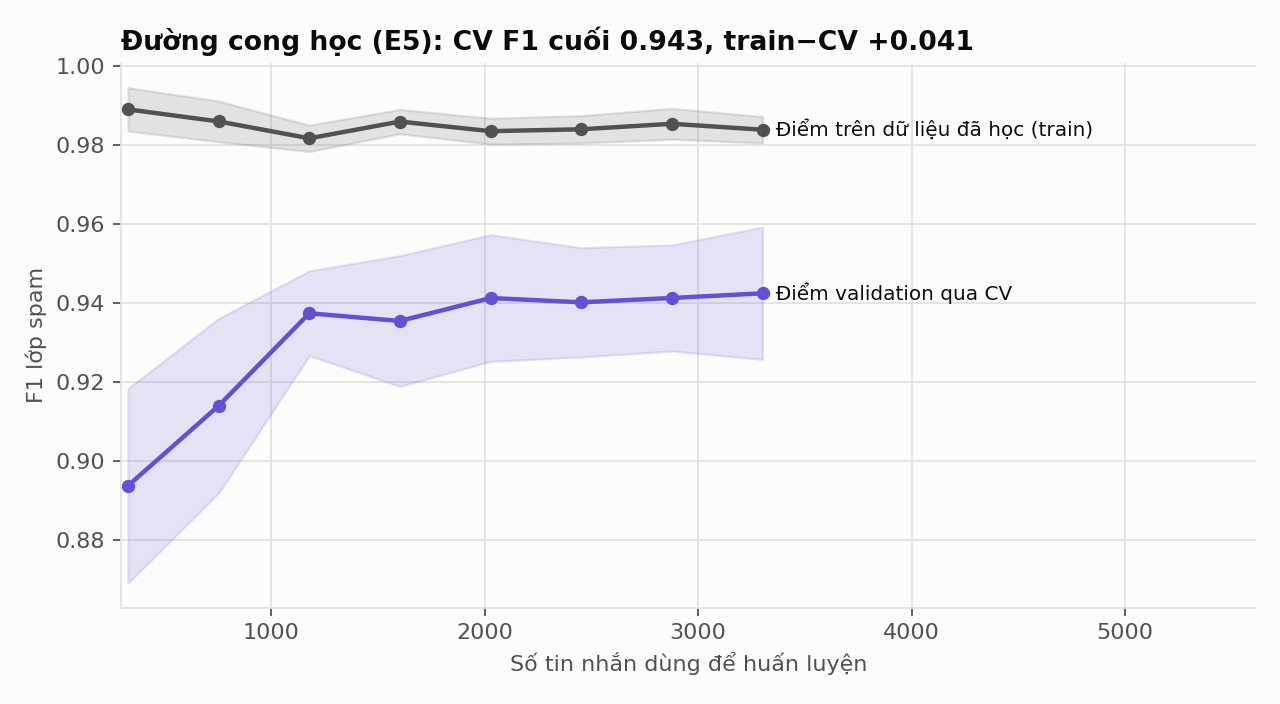
\includegraphics[width=0.9\textwidth]{images/viz_9_learning_curve.png}
    \caption{Đường cong học của E5 (F1 lớp spam theo số mẫu huấn luyện)}
    \label{fig:learning-curve}
    \Nguon{Nhóm xây dựng bằng lệnh \texttt{python -m spam\_filter check}}
\end{figure}

\section{Kiểm tra rò rỉ dữ liệu và học thuộc}
\label{sec:sanity}

Một kết quả F1 trên 0,94 cho bài toán lọc spam dễ khiến người đọc nghi ngờ. Nhóm vì vậy cài đặt chín phép kiểm tra tự động cho mô hình E5 (Bảng~\ref{tab:sanity}).

\begin{table}[H]
\centering
\caption{Kết quả các phép kiểm tra rò rỉ, học thuộc và baseline đơn giản (mô hình E5)}
\label{tab:sanity}
\small
\begin{tabular}{|p{6.1cm}|p{4.6cm}|c|}
\hline
\textbf{Phép kiểm tra} & \textbf{Kết quả} & \textbf{Trạng thái} \\
\hline
A1. Tin trùng chính xác giữa train và test & 0 (yêu cầu $=0$) & OK \\
\hline
A2. Trùng sau chuẩn hóa chữ hoa/thường, dấu câu & 8 (yêu cầu $=0$) & Lưu ý \\
\hline
A3. Tin test có bản gần giống (cosine $\ge0{,}8$) trong train & 65 tin (6,3\%) & OK \\
\hline
A4. F1 trên tin ``mới'' (không có bản gần giống) & 0,912 (toàn test 0,944; giảm 0,031) & OK \\
\hline
A5. Xáo trộn nhãn train rồi đo trên test (5 lần) & F1 trung bình 0,105 & OK \\
\hline
B1. Chênh lệch F1 train $-$ test & $0{,}983-0{,}944=0{,}040$ & OK \\
\hline
B2. F1 CV (train) so với test & 0,943 so với 0,944 & OK \\
\hline
C1. Baseline chỉ dùng độ dài và số chữ số & F1 0,886 (mô hình hơn 0,057) & OK \\
\hline
C2. Đoán ngẫu nhiên theo tỉ lệ lớp & F1 0,083 & OK \\
\hline
\end{tabular}
\Nguon{Nhóm thực nghiệm (lệnh \texttt{python -m spam\_filter check}); kết quả: 8 OK, 1 lưu ý, 0 lỗi}
\end{table}

Diễn giải theo từng nhóm:

\begin{itemize}
    \item \textbf{Rò rỉ (A).} Không có tin trùng chính xác giữa hai tập. Tám tin trùng \textit{sau khi chuẩn hóa} (khác nhau chỉ ở chữ hoa/dấu câu) là một ``lưu ý'' nhỏ, chiếm dưới 1\% tập kiểm tra. Khi chỉ xét các tin test \textit{không} có bản gần giống trong train (A4), F1 giảm 0,031 xuống 0,912, nghĩa là một phần nhỏ điểm số đến từ các tin gần trùng nhưng phần lớn vẫn là khả năng khái quát hóa thực. Phép xáo trộn nhãn (A5) cho F1 xấp xỉ 0,105, tức mô hình trở về mức đoán mò khi nhãn mất ý nghĩa, một chứng cứ mạnh rằng pipeline \textit{không} ``nhìn trộm'' nhãn.
    \item \textbf{Học thuộc (B).} Chênh lệch train--test (0,040) thấp, và CV trên train (0,943) khớp tập test (0,944).
    \item \textbf{Bài toán có thật sự khó không (C).} Baseline chỉ dùng độ dài và số chữ số đã đạt F1 0,886, nên bài toán trên corpus này \textit{tương đối dễ}: một phần lớn tín hiệu nằm ở đặc điểm cấu trúc. Mô hình NB hơn baseline đơn giản này 0,057 F1; đó là mức cải thiện có thật nhưng khiêm tốn, cần được nhìn nhận khi đánh giá ``độ khó'' của bài toán.
\end{itemize}

Một cảnh báo quan trọng: các phép kiểm tra này loại trừ rò rỉ \textit{trong nội bộ corpus}, không loại trừ \textit{thiên lệch nguồn} (ham chủ yếu từ Singapore, spam từ Vương quốc Anh; xem Mục~1.4). Mô hình có thể một phần dựa vào dấu hiệu nguồn gốc như phương ngữ.

\section{Ảnh hưởng của ngưỡng quyết định}

Mặc định mô hình gọi một tin là spam khi $P(\text{spam}\mid d)\ge0{,}5$. Vì chi phí của FP và FN khác nhau (Mục~1.6), nhóm khảo sát việc đổi ngưỡng cho E5 (Bảng~\ref{tab:nguong}, Hình~\ref{fig:nguong}).

\begin{table}[H]
\centering
\caption{Precision, Recall, F1 và số lỗi của E5 theo ngưỡng quyết định (tập kiểm tra)}
\label{tab:nguong}
\begin{tabular}{|c|c|c|c|c|c|}
\hline
\textbf{Ngưỡng} & \textbf{Precision} & \textbf{Recall} & \textbf{F1} & \textbf{FP} & \textbf{FN} \\
\hline
0,3 & 0,9528 & 0,9453 & 0,9490 & 6 & 7 \\
\hline
0,4 & 0,9754 & 0,9297 & 0,9520 & 3 & 9 \\
\hline
\textbf{0,5 (mặc định)} & 0,9750 & 0,9141 & 0,9435 & 3 & 11 \\
\hline
0,6 & 0,9912 & 0,8828 & 0,9339 & 1 & 15 \\
\hline
0,7 & 0,9912 & 0,8750 & 0,9295 & 1 & 16 \\
\hline
0,8 & 0,9910 & 0,8594 & 0,9205 & 1 & 18 \\
\hline
0,9 & 0,9907 & 0,8359 & 0,9068 & 1 & 21 \\
\hline
\end{tabular}
\Nguon{Nhóm thực nghiệm}
\end{table}

\begin{figure}[H]
    \centering
    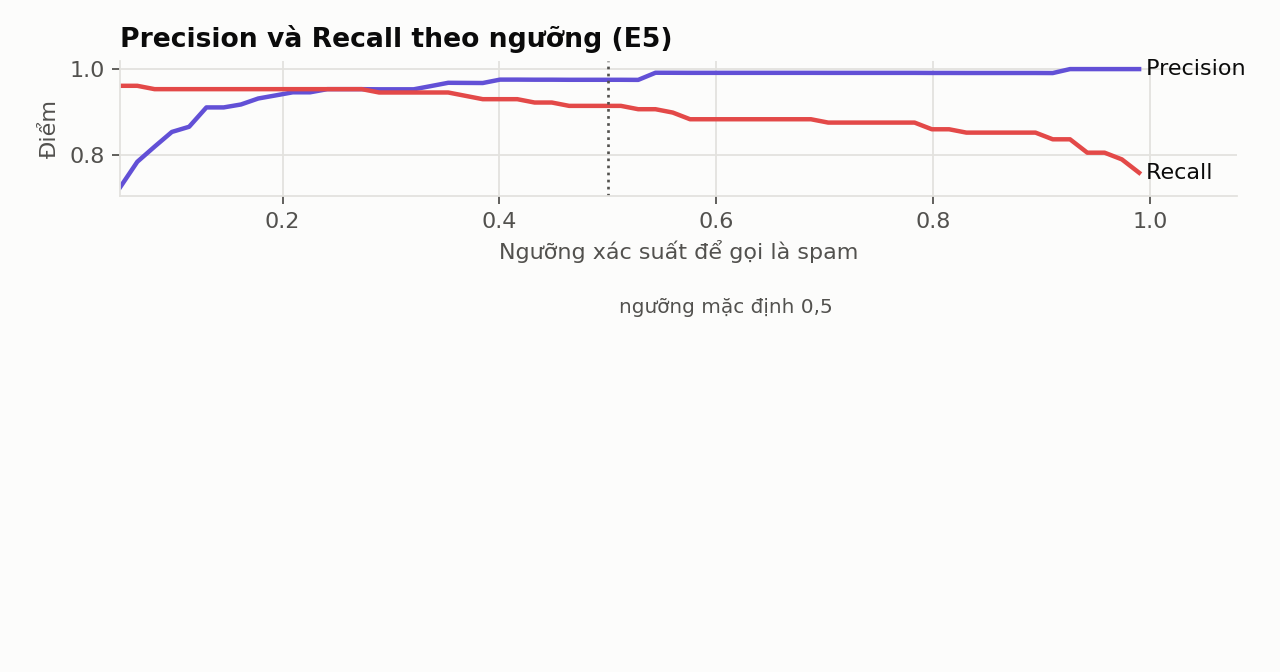
\includegraphics[width=0.85\textwidth]{images/viz_7_threshold_tradeoff.png}
    \caption{Đường Precision và Recall của E5 theo ngưỡng xác suất}
    \label{fig:nguong}
    \Nguon{Nhóm xây dựng từ kết quả thí nghiệm}
\end{figure}

Tăng ngưỡng từ 0,5 lên 0,6 giảm FP từ 3 xuống 1 nhưng làm FN tăng từ 11 lên 15; từ 0,6 trở đi hầu như không còn giảm được FP nào nữa (vẫn còn 1 tin ham bị chặn) trong khi FN tiếp tục tăng. Điều này cho thấy tin ham còn sót lại là tin mô hình \textit{rất tự tin} nhầm lẫn, ngưỡng không giải quyết được. \textbf{Lưu ý phương pháp}: các giá trị ở Bảng~\ref{tab:nguong} được đọc trên tập kiểm tra nên chỉ mang tính \textit{mô tả}; nếu triển khai thật, ngưỡng phải được chọn bằng CV trên tập huấn luyện hoặc một tập validation riêng, rồi mới đánh giá một lần trên tập test.

\chapter{PHÂN TÍCH LỖI VÀ DIỄN GIẢI MÔ HÌNH}

Chương này phân tích 14 tin bị phân loại sai của mô hình E5 trên tập kiểm tra (3 FP và 11 FN) và xem mô hình đã ``học'' những gì. Với mỗi lỗi, nhóm tính đóng góp của từng đặc trưng vào quyết định, tức tích giữa giá trị TF-IDF của đặc trưng và hiệu số log xác suất $\ln P(w\mid\text{spam})-\ln P(w\mid\text{ham})$ của Naive Bayes. Đóng góp dương đẩy tin về phía spam, đóng góp âm đẩy về phía ham.

\section{Phân tích các tin ham bị chặn nhầm (FP)}

Mô hình chặn nhầm \textbf{3 tin hợp lệ} (Bảng~\ref{tab:fp}); đây là loại lỗi nghiêm trọng hơn theo tiêu chí ở Mục~1.6.

\begin{table}[H]
\centering
\caption{Các tin ham bị dự đoán nhầm là spam (FP) của E5}
\label{tab:fp}
\begin{tabular}{|p{4.8cm}|c|p{6.6cm}|}
\hline
\textbf{Nội dung tin} & \textbf{$P(\text{spam})$} & \textbf{Đặc trưng đẩy về spam} \\
\hline
\textit{``Nokia phone is lovly..''} & 0,922 & \textit{nokia}, \textit{nokia phone} (đóng góp lớn nhất). \\
\hline
\textit{``K:)eng rocking in ashes:)''} & 0,541 & \textit{eng} (chỉ có 2 đặc trưng trong tin). \\
\hline
\textit{``Unlimited texts. Limited minutes.''} & 0,539 & \textit{unlimited}, \textit{texts}. \\
\hline
\end{tabular}
\Nguon{Nhóm phân tích từ \texttt{outputs/results/errors\_E5.csv}}
\end{table}

Ba nhận xét:

\begin{enumerate}[label=(\arabic*)]
    \item \textbf{Cả ba tin đều rất ngắn} (22--33 ký tự, chỉ 2--5 đặc trưng). Với tin quá ngắn, một từ duy nhất có thể chi phối cả quyết định; tin thứ hai bị chặn gần như chỉ vì từ \textit{eng}.
    \item \textbf{Hiện tượng ``từ khóa gây hiểu lầm''.} \textit{Nokia} nằm trong nhóm từ đặc trưng spam mạnh nhất (Bảng~\ref{tab:top-words}) vì trong dữ liệu có nhiều spam quảng cáo điện thoại Nokia. Mô hình không biết một lời nhận xét về chiếc điện thoại thì vô hại; nó chỉ thấy từ khóa.
    \item \textbf{Hai trong ba FP chỉ ở sát ranh giới} (xác suất 0,54). Khi tăng ngưỡng lên 0,6 chúng được cứu (Bảng~\ref{tab:nguong}: FP giảm từ 3 xuống 1), chỉ còn tin \textit{``Nokia phone is lovly..''} với xác suất 0,92 là lỗi ``tự tin''.
\end{enumerate}

\section{Phân tích các tin spam bị bỏ lọt (FN)}

Mô hình bỏ lọt \textbf{11 tin spam}. Nhóm phân loại chúng theo kiểu ngôn ngữ (Bảng~\ref{tab:fn}). Một số tin có nội dung người lớn nên chỉ được mô tả khái quát.

\begin{table}[H]
\centering
\caption{Phân nhóm các tin spam bị bỏ lọt (FN) của E5}
\label{tab:fn}
\small
\begin{tabular}{|>{\raggedright\arraybackslash}p{3.2cm}|c|>{\raggedright\arraybackslash}p{5.8cm}|>{\raggedright\arraybackslash}p{3cm}|}
\hline
\textbf{Nhóm} & \textbf{Số tin} & \textbf{Đặc điểm và ví dụ rút gọn} & \textbf{$P(\text{spam})$} \\
\hline
Mạo danh tin nhắn cá nhân (lừa gọi lại / bắt chuyện) & 3 & \textit{``Sorry I missed your call let's talk when you have the time. I'm on 0709...''}; tin hỏi thăm về trang web cá nhân; tin ``\textit{dating:...}'' như lời kể chuyện. & 0,003; 0,075; 0,006 \\
\hline
Tin quảng cáo dịch vụ người lớn, văn phong thân mật & 4 & Dùng ngôn ngữ hội thoại (\textit{babe}, \textit{me}, \textit{u}), đuôi chỉ dẫn \textit{txt}/\textit{STOP}, mức cước (\textit{150ppmsg}). & 0,004; 0,012; 0,363; 0,378 \\
\hline
Dịch vụ thuê bao, thông báo thanh toán & 2 & Dịch vụ tử vi/chiêm tinh (\textit{Reply ANS}, \textit{Reply END}); thông báo ``bị tính 35p'' mua clip video. & 0,427; 0,448 \\
\hline
Quảng cáo gắn tên miền & 2 & Tin ``\textit{Cashbin.co.uk ... cash give away}'' (dài, văn phong khuyến mãi nhẹ); tin giới thiệu dịch vụ gửi tin ẩn danh \textit{thesmszone.com}. & 0,286; 0,037 \\
\hline
\end{tabular}
\Nguon{Nhóm phân tích từ \texttt{outputs/results/errors\_E5.csv}}
\end{table}

Phân bố xác suất của các FN cho thấy hai kiểu lỗi khác hẳn nhau về bản chất:

\begin{itemize}
    \item \textbf{5/11 lỗi nằm ở vùng ranh giới} ($P=0{,}29$--$0{,}45$): mô hình ``nghi ngờ'' nhưng chưa đủ. Đây là các lỗi có thể giảm bằng cách hạ ngưỡng. Quả thật ở ngưỡng 0,3 tổng FN giảm từ 11 xuống 7 (Bảng~\ref{tab:nguong}) nhưng phải trả giá bằng FP tăng từ 3 lên 6.
    \item \textbf{6/11 lỗi là ``chắc chắn sai''} ($P\le0{,}075$): các spam này được viết như tin nhắn cá nhân bình thường, hầu như không chứa từ khóa khuyến mãi điển hình. Với mô hình dựa trên túi từ, chúng \textit{không thể phân biệt được} khỏi ham, vì dấu hiệu duy nhất là ý đồ (nhờ gọi lại một số lạ, dẫn tới trang web), thuộc về ngữ nghĩa và ngữ cảnh. Hạ ngưỡng không giúp ích; cần đặc trưng khác hoặc mô hình hiểu ngữ nghĩa.
\end{itemize}

Ví dụ điển hình: tin \textit{``Sorry I missed your call let's talk when you have the time. I'm on 07090201529''} có các đặc trưng đẩy về ham mạnh (\textit{sorry}, \textit{let}, \textit{have the}) lấn át tín hiệu số điện thoại (\texttt{numtoken}), dẫn tới $P(\text{spam})=0{,}003$. Việc token hóa số điện thoại giúp mô hình nhận ra \textit{``có một số''}, nhưng một số điện thoại trong ham (ví dụ ``gọi tôi theo số...'') cũng xuất hiện, nên tín hiệu này không đủ độc lập.

\section{Mô hình đã học điều gì?}

Vì Naive Bayes khả diễn giải, nhóm xếp hạng các n-gram theo hiệu số $\ln P(w\mid\text{spam})-\ln P(w\mid\text{ham})$ trong E5 (Bảng~\ref{tab:top-words}).

\begin{table}[H]
\centering
\caption{Các n-gram có điểm phân biệt cao nhất cho từng lớp (E5)}
\label{tab:top-words}
\small
\begin{tabular}{|c|p{3.6cm}|c|p{3.2cm}|c|}
\hline
\textbf{Hạng} & \textbf{Đặc trưng spam} & \textbf{Điểm} & \textbf{Đặc trưng ham} & \textbf{Điểm} \\
\hline
1 & \textit{claim} & 5,84 & \textit{gt} & $-4,49$ \\
\hline
2 & \textit{prize} & 5,72 & \textit{lt} & $-4,49$ \\
\hline
3 & \textit{numtoken now} & 5,65 & \textit{lt gt} & $-4,40$ \\
\hline
4 & \textit{nokia} & 5,38 & \textit{lor} & $-4,32$ \\
\hline
5 & \textit{numtoken moneytoken} & 5,35 & \textit{da} & $-4,28$ \\
\hline
6 & \textit{box numtoken} & 5,26 & \textit{he} & $-4,26$ \\
\hline
7 & \textit{your mobile} & 5,26 & \textit{she} & $-3,91$ \\
\hline
8 & \textit{have won} & 5,24 & \textit{later} & $-3,86$ \\
\hline
9 & \textit{moneytoken cash} & 5,19 & \textit{lol} & $-3,76$ \\
\hline
10 & \textit{to claim} & 5,18 & \textit{anything} & $-3,72$ \\
\hline
\end{tabular}
\Nguon{Nhóm tính từ \texttt{outputs/results/top\_words\_E5.csv}}
\end{table}

Có ba quan sát có giá trị:

\begin{enumerate}[label=(\arabic*)]
    \item \textbf{Phía spam đúng với trực giác} và xác nhận giả thuyết H1: kêu gọi hành động (\textit{claim}, \textit{to claim}), phần thưởng (\textit{prize}, \textit{have won}), và \textit{các token cấu trúc} do tiền xử lý tạo ra (\textit{numtoken now}, \textit{numtoken moneytoken}, \textit{moneytoken cash}, \textit{box numtoken}). Bốn trên mười đặc trưng hàng đầu là cụm có token hóa; điều này giải thích tại sao token hóa giúp ích (Mục~\ref{sec:nhay-tham-so}): nó biến các giá trị duy nhất thành các đặc trưng lặp lại và có tính phân biệt.
    \item \textbf{Phía ham chứa ``dấu vân tay'' của nguồn dữ liệu.} \textit{gt}, \textit{lt}, \textit{lt gt} là phần còn lại của chuỗi thực thể HTML \texttt{\&lt;\#\&gt;} trong corpus gốc, hoàn toàn không liên quan tới ý nghĩa; \textit{lor} và \textit{da} là tiểu từ đặc trưng của tiếng Anh Singapore/Nam Á trong tin nhắn của sinh viên. Đây là \textbf{bằng chứng trực tiếp cho thiên lệch nguồn} đã cảnh báo ở Mục~1.4: một phần ``hiểu biết'' của mô hình là nhận ra phương ngữ và định dạng thay vì bản chất spam. Mô hình sẽ dễ sai khi gặp ham viết bằng văn phong khác hoặc spam kiểu mới.
    \item \textbf{Từ trung tính vẫn có trọng số.} \textit{he}, \textit{she}, \textit{later}, \textit{anything} nghiêng mạnh về ham, nhất quán với ý rằng tin cá nhân nhắc đến người thứ ba và thời gian. Đây cũng là lý do một số spam viết như tin cá nhân (nhóm FN thứ nhất) rất khó bị phát hiện.
\end{enumerate}

\section{Liên hệ với giả định của mô hình và đặc điểm dữ liệu}

\begin{itemize}
    \item \textbf{Giả định độc lập có điều kiện.} Các cụm như \textit{to claim}, \textit{have won} được đếm \textit{vừa} như hai từ đơn \textit{vừa} như một bigram, nên cùng một bằng chứng bị tính trùng; điều này làm xác suất đầu ra quá tự tin (nhiều FP/FN có xác suất cực đoan như 0,003 hoặc 0,922) và là lý do không nên diễn giải $P(\text{spam})$ như xác suất đã hiệu chuẩn.
    \item \textbf{Mất cân bằng lớp.} Xác suất tiên nghiệm spam chỉ 12,45\% làm mô hình thiên về dự đoán ham khi bằng chứng không rõ; điều này góp phần vào nhóm FN ranh giới. Có thể bù bằng hạ ngưỡng hoặc điều chỉnh tiên nghiệm.
    \item \textbf{Tin ngắn.} Cả ba FP đều rất ngắn; với ít đặc trưng, một từ hiếm có thể chi phối. Tin ngắn là vùng rủi ro đặc biệt của mô hình túi từ.
    \item \textbf{Dữ liệu trùng lặp.} Nếu giữ nguyên 414 tin trùng, mô hình sẽ đếm một số mẫu spam nhiều lần và các phép đánh giá có thể bị làm đẹp; việc loại trùng trước khi chia là cần thiết để lỗi quan sát được có ý nghĩa.
\end{itemize}

\section{Đề xuất cải thiện dựa trên bằng chứng}

Các đề xuất dưới đây được gắn trực tiếp với lỗi quan sát được.

\begin{table}[H]
\centering
\caption{Đề xuất cải thiện và căn cứ}
\label{tab:de-xuat}
\small
\begin{tabular}{|p{3.7cm}|p{5.3cm}|p{5cm}|}
\hline
\textbf{Đề xuất} & \textbf{Căn cứ từ thực nghiệm} & \textbf{Kỳ vọng và rủi ro} \\
\hline
Chọn ngưỡng bằng CV, ưu tiên Precision & 2/3 FP chỉ ở ranh giới; 5/11 FN ở ranh giới; ngưỡng 0,6 giảm FP còn 1 (Bảng~\ref{tab:nguong}). & Giảm chặn nhầm; đánh đổi Recall. Phải chọn trên validation. \\
\hline
Hiệu chuẩn xác suất (Platt/isotonic) hoặc dùng \texttt{class\_weight}/prior & Xác suất đầu ra cực đoan; lỗi tự tin 0,922 và 0,003. & Ngưỡng có ý nghĩa xác suất thật. \\
\hline
Đặc trưng thủ công: độ dài, số chữ số, tỉ lệ chữ hoa, có URL & Baseline độ dài + chữ số đã có F1 0,886 (Mục~\ref{sec:sanity}); nhiều tín hiệu nằm ngoài từ vựng. & Bổ sung thông tin độc lập với từ; cần mô hình kết hợp (ví dụ hồi quy logistic). \\
\hline
N-gram ký tự và chuẩn hóa viết tắt SMS & Nhiều viết tắt/viết sai (\textit{u}, \textit{2day}, \textit{lovly}); \textit{eng} gây FP. & Giảm từ ngoài từ vựng; tăng chi phí. \\
\hline
Thêm dữ liệu spam hiện đại và đa nguồn & Thiên lệch nguồn (\textit{lor}, \textit{gt}); đường cong học đi ngang. & Cải thiện khái quát hóa; cần gán nhãn. \\
\hline
Biểu diễn ngữ nghĩa (sentence embedding) & 6/11 FN là spam ``giả cá nhân''. & Có thể bắt ý đồ; tốn tài nguyên, giảm khả năng giải thích. \\
\hline
\end{tabular}
\Nguon{Nhóm tổng hợp}
\end{table}

Các đề xuất này \textit{chưa được kiểm chứng bằng thực nghiệm} trong khuôn khổ bài tập lớn; chúng là hướng phát triển có căn cứ, không phải kết quả đã đạt.

\chapter{ỨNG DỤNG THỰC TẾ VÀ SẢN PHẨM DEMO}

\section{Ứng dụng web demo}

Để minh họa mô hình hoạt động end-to-end, nhóm xây dựng ứng dụng web bằng Streamlit (tệp \texttt{app.py}). Ứng dụng đọc mô hình và kết quả đã lưu trong thư mục \texttt{outputs/}, nên \textit{không} huấn luyện lại khi mở, và đi theo đúng luồng của báo cáo: Demo dự đoán, Nguồn dữ liệu, EDA, Tiền xử lý, Đặc trưng, Mô hình, Đánh giá, Phân tích lỗi, Kết luận.

Các chức năng chính của trang Demo:

\begin{itemize}
    \item \textbf{Dự đoán một tin nhắn}: nhập văn bản tiếng Anh, nhận nhãn spam/ham kèm xác suất.
    \item \textbf{Kéo ngưỡng quyết định} (từ 0,05 đến 0,95): quan sát trực tiếp đánh đổi giữa chặn nhầm và bỏ lọt (xem Mục~5.5).
    \item \textbf{Giải thích dự đoán}: hiển thị những từ đẩy tin về phía spam hoặc ham, dựa trên đóng góp của đặc trưng như ở Chương~6.
    \item \textbf{Kiểm thử hàng loạt}: mỗi dòng là một tin, có thể gắn tiền tố \texttt{spam|} hoặc \texttt{ham|} để ứng dụng tự chấm đúng/sai.
\end{itemize}

Cách chạy (sau khi đã huấn luyện, Phụ lục~1):

\begin{verbatim}
python -m spam_filter run
streamlit run app.py
\end{verbatim}

Ứng dụng cũng hỗ trợ dự đoán qua dòng lệnh: \texttt{python -m spam\_filter predict "Free entry! Call 0906... to win £500"}.

\section{Khuyến nghị triển khai}

Từ các kết quả ở Chương~5 và~6, nhóm đưa ra các khuyến nghị cho một bộ lọc SMS thực tế. Khuyến nghị nào chưa được kiểm chứng bằng thực nghiệm đều được ghi rõ.

\subsection{Chọn mô hình}

\begin{itemize}
    \item \textbf{Dùng họ Naive Bayes làm mô hình cơ sở}: kết quả vượt K-NN và Cây quyết định ở mọi lần chia (Mục~5.3), huấn luyện chỉ mất vài giây, dự đoán nhanh và khả diễn giải. Giữa E0 (BoW), E2 và E5, khác biệt nằm trong dải nhiễu của phép đo, nên có thể ưu tiên cấu hình đơn giản nhất mà vẫn đạt mức tương đương; token hóa số/tiền/URL vẫn là một bước rẻ và có cơ sở lý thuyết.
    \item \textbf{Không dùng K-NN cho triển khai trực tuyến}: chi phí dự đoán tăng theo kích thước tập huấn luyện và chất lượng thấp hơn.
\end{itemize}

\subsection{Chính sách ngưỡng theo chi phí lỗi}

Thay vì ngưỡng 0,5 mặc định, nên thiết kế \textbf{chính sách ba mức} dựa trên xác suất, phù hợp với việc FP nặng hơn FN:

\begin{table}[H]
\centering
\caption{Đề xuất chính sách xử lý theo xác suất spam}
\label{tab:chinh-sach}
\begin{tabular}{|p{3.4cm}|p{4.2cm}|p{6.2cm}|}
\hline
\textbf{Xác suất spam} & \textbf{Hành động} & \textbf{Lý do} \\
\hline
$\ge 0{,}9$ & Chặn hoặc chuyển vào hộp thư rác & Mô hình rất tự tin; ở ngưỡng 0,9 chỉ còn 1 FP trên tập kiểm tra. \\
\hline
$0{,}3$ -- $0{,}9$ & Gắn cảnh báo ``nghi là spam'' nhưng vẫn giao tin & Vùng ranh giới chứa 2/3 FP và 4/11 FN của E5 trên tập kiểm tra; không nên chặn thẳng. \\
\hline
$< 0{,}3$ & Giao bình thường & Rủi ro chặn nhầm tin quan trọng lớn hơn lợi ích; 7/11 FN nằm ở đây và cần biện pháp khác (Mục~6.2). \\
\hline
\end{tabular}
\Nguon{Nhóm đề xuất dựa trên Bảng~\ref{tab:nguong}; các mức cụ thể cần được hiệu chỉnh trên tập validation}
\end{table}

Các mốc 0,3 và 0,9 được rút ra từ quan sát trên tập kiểm tra nên chỉ là \textbf{điểm khởi đầu}; khi triển khai cần chọn bằng validation theo chi phí kinh doanh thực tế (ví dụ chi phí một tin OTP bị chặn so với chi phí một khiếu nại spam).

\subsection{Giám sát và vòng đời mô hình}

\begin{itemize}
    \item \textbf{Spam thay đổi theo thời gian} (concept drift): cần giám sát tỉ lệ spam và phân bố xác suất, huấn luyện lại định kỳ với dữ liệu mới gán nhãn.
    \item \textbf{Vòng lặp phản hồi}: cho phép người dùng báo ``đây là spam''/``không phải spam'' và đưa vào dữ liệu huấn luyện; đặc biệt ưu tiên các tin FP vì chi phí cao.
    \item \textbf{Quy tắc bổ sung}: kết hợp danh sách chặn/cho phép (số điện thoại, đầu số đã biết) với mô hình để bù các lỗi ``chắc chắn sai'' mà mô hình văn bản không thể bắt (Mục~6.2).
    \item \textbf{Quyền riêng tư}: nội dung SMS là dữ liệu nhạy cảm; nên xử lý trên thiết bị hoặc ẩn danh hóa trước khi lưu để huấn luyện.
\end{itemize}

\subsection{Phạm vi áp dụng và các giới hạn cần nêu rõ}

Mô hình hiện tại \textbf{chỉ phù hợp với tin nhắn tiếng Anh} và đã được đánh giá trên một corpus cũ có thiên lệch nguồn. Không nên triển khai trực tiếp cho tin nhắn tiếng Việt hoặc cho spam hiện đại (liên kết rút gọn, giả mạo ngân hàng, mã xác thực) mà không huấn luyện lại và đánh giá trên dữ liệu đại diện. Con số F1 94\% trong báo cáo \textit{mô tả corpus này}, không phải tiên đoán chất lượng ngoài thực tế.


% =========================
% PHẦN CUỐI BÁO CÁO
% =========================
\clearpage
\UnnumberedChapter{KẾT LUẬN}

\textbf{Kết quả đạt được.} Báo cáo đã xây dựng và đánh giá một pipeline phân loại tin nhắn rác hoàn chỉnh trên bộ dữ liệu SMS Spam Collection, từ dữ liệu thô đến ứng dụng demo. Pipeline loại 414 tin trùng trước khi chia, chia 80/20 có phân tầng với \texttt{random\_state}=42, ghép làm sạch, vector hóa và mô hình trong một \texttt{Pipeline} để vectorizer chỉ được \texttt{fit} trên tập huấn luyện, chọn mô hình bằng F1 lớp spam qua CV 5 fold trên tập huấn luyện. Bảy thí nghiệm (một baseline, các biến thể biểu diễn, ba thuật toán và hai thí nghiệm đối chứng tiền xử lý) được chạy và ghi log tham số.

\textbf{Mô hình tốt nhất.} Cấu hình E5 (token hóa URL/tiền/số, bỏ dấu câu, TF-IDF $(1,2)$-gram với \texttt{min\_df}=2, Multinomial Naive Bayes với $\alpha=0{,}1$) đạt trên tập kiểm tra Accuracy 98,64\%, Precision 97,50\%, Recall 91,41\%, F1 lớp spam 94,35\% và ROC-AUC 0,9905, với 3 tin ham bị chặn nhầm và 11 tin spam bị bỏ lọt trong 1\,032 tin.

\textbf{Các kết luận có bằng chứng vững.}
\begin{enumerate}[label=(\arabic*)]
    \item \textbf{Naive Bayes vượt K-NN và Decision Tree một cách ổn định}: khoảng cách F1 ($0{,}04$--$0{,}11$) lặp lại ở cả 10 lần chia ngẫu nhiên và lớn hơn nhiều độ dao động của phép đo.
    \item \textbf{Accuracy là thước đo gây hiểu lầm}: mô hình luôn đoán ``ham'' đã đạt 87,6\%, và mọi mô hình đều có Accuracy 97--98,6\%, trong khi Recall của lớp spam chênh nhau tới 13 điểm phần trăm.
    \item \textbf{Tham số làm mượt $\alpha$ có tác động lớn nhất}: với TF-IDF, $\alpha\ge0{,}5$ làm CV F1 sụt từ 0,943 xuống 0,912 rồi 0,860; mặc định của BoW không chuyển được sang TF-IDF.
    \item \textbf{Token hóa số là bước tiền xử lý hữu ích nhất} ($+0{,}013$ CV F1), phù hợp với EDA (76,5\% spam chứa chuỗi từ 5 chữ số trở lên so với 0,1\% ham).
    \item \textbf{Không có dấu hiệu rò rỉ hay học thuộc nghiêm trọng}: không trùng chính xác train/test; F1 giảm chỉ 0,031 trên các tin test không có bản gần giống; xáo trộn nhãn đưa F1 về 0,105; CV (0,943) khớp test (0,944).
\end{enumerate}

\textbf{Các kết luận cần được hiểu thận trọng.} Việc BoW so với TF-IDF, unigram so với bigram, và có/không bỏ stopword \textit{không} tạo ra khác biệt có thể phân biệt được khỏi nhiễu trên dữ liệu này (chênh lệch $\le0{,}01$ so với độ lệch chuẩn 0,012--0,019 khi đổi cách chia). Ưu thế của E5 so với E0 là nhỏ ($+0{,}007\pm0{,}008$, thắng 7/10 lần chia) và nhóm không tuyên bố ý nghĩa thống kê. Các thí nghiệm độ nhạy cho thấy một số cấu hình đơn giản hơn cho CV F1 tương đương hoặc cao hơn E5.

\textbf{Hạn chế.}
\begin{itemize}
    \item \textbf{Dữ liệu}: chỉ tiếng Anh, cũ, nhỏ (5\,160 tin sau khử trùng); ham và spam đến từ các nguồn khác nhau nên mô hình học một phần dấu hiệu nguồn (\textit{lor}, \textit{da}, \textit{lt gt}); kết quả không chứng minh khả năng tổng quát hóa sang SMS hiện đại.
    \item \textbf{Đánh giá}: tập kiểm tra chỉ có 128 spam nên mỗi lỗi thay đổi F1 khoảng 0,4 điểm phần trăm; các giá trị ngưỡng ở Bảng~\ref{tab:nguong} được đọc trên tập kiểm tra nên chỉ mang tính mô tả; không khóa phiên bản thư viện.
    \item \textbf{Mô hình}: giả định độc lập của Naive Bayes làm xác suất kém hiệu chuẩn; mô hình không bắt được nhóm spam ``giả tin nhắn cá nhân'' (6/11 lỗi bỏ lọt là lỗi chắc chắn sai).
    \item \textbf{Phạm vi}: chưa thử các mô hình tuyến tính như hồi quy logistic hoặc SVM, và chưa thử mô hình học sâu.
\end{itemize}

\textbf{Hướng phát triển.} Dựa trên lỗi quan sát được (Bảng~\ref{tab:de-xuat}): (i) chọn ngưỡng bằng validation và hiệu chuẩn xác suất; (ii) bổ sung đặc trưng cấu trúc và n-gram ký tự, thử hồi quy logistic/SVM tuyến tính trên cùng biểu diễn; (iii) mở rộng dữ liệu bằng spam hiện đại, đa ngôn ngữ (đặc biệt tiếng Việt) và đa nguồn để giảm thiên lệch; (iv) thử biểu diễn ngữ nghĩa (sentence embedding) cho nhóm spam viết như tin cá nhân; (v) giám sát concept drift và thiết lập vòng lặp phản hồi khi triển khai.

Bài tập lớn giúp nhóm củng cố một bài học xuyên suốt: \textit{độ tin cậy của một con số kết quả quan trọng không kém con số đó cao đến đâu}. Việc chống rò rỉ dữ liệu, chọn thước đo đúng với chi phí nghiệp vụ, đo độ dao động khi đổi cách chia, và nói rõ giới hạn của dữ liệu là những thực hành nhóm sẽ tiếp tục áp dụng trong các bài toán học máy sau này.


\clearpage
\appendix
\UnnumberedChapter{PHỤ LỤC}

% Đánh số hình/bảng trong phụ lục dạng PL.1, PL.2 (chương không đánh số nên không dùng số chương).
\renewcommand{\thetable}{PL.\arabic{table}}
\renewcommand{\thefigure}{PL.\arabic{figure}}
\setcounter{table}{0}\setcounter{figure}{0}

\section*{Phụ lục 1. Hướng dẫn tái lập kết quả}

\textbf{Yêu cầu:} Python $\ge3{,}10$. Môi trường nhóm dùng để sinh số liệu trong báo cáo: Python 3.14.6, scikit-learn 1.9.0, NumPy 2.4.1, pandas 3.1.0 (xem Bảng~\ref{tab:moi-truong}).

\begin{verbatim}
pip install -r requirements.txt

python -m spam_filter eda      # thống kê và biểu đồ EDA
python -m spam_filter run      # chạy E0..E6, lưu mô hình, bảng, lỗi
python -m spam_filter viz      # bộ biểu đồ cho báo cáo (viz_*.png)
python -m spam_filter viz --stability   # lặp 10 random_state
python -m spam_filter check    # kiểm tra rò rỉ / học thuộc / baseline
python -m spam_filter predict "Free entry! Call to win 500"
pytest                         # 41 kiểm thử
streamlit run app.py           # ứng dụng demo
\end{verbatim}

\textbf{Thứ tự khuyến nghị:} \texttt{eda} $\to$ \texttt{run} $\to$ \texttt{viz} $\to$ \texttt{check} $\to$ \texttt{streamlit run app.py}. Thư mục \texttt{outputs/} không được đưa lên git vì sinh lại được bằng các lệnh trên. Các hình trong thư mục \texttt{reports/images/} của báo cáo được sao chép từ \texttt{outputs/figures/}.

\textbf{Về phép đo độ nhạy (Bảng~\ref{tab:nhay}, \ref{tab:ablation}) và ngưỡng (Bảng~\ref{tab:nguong}).} Các bảng này được sinh bằng một đoạn mã tạm thời gọi lại chính các mô-đun của \texttt{spam\_filter} (\texttt{TextCleaner}, \texttt{build\_vectorizer}, \texttt{cross\_val\_f1}) với cùng cách chia dữ liệu và \texttt{random\_state}=42; đoạn mã này chưa được đưa vào kho mã nguồn dưới dạng lệnh CLI.

\textbf{Ghi chú về phiên bản.} Phiên bản README trước đây của dự án ghi E3 ROC-AUC 0,9682 và E5 CV F1 0,9414. Khi chạy lại với mã hiện tại, E3 cho 0,9685 và E5 cho 0,9425 (do bước nhận diện URL được cải tiến); báo cáo này dùng các số mới.

\section*{Phụ lục 2. Ma trận nhầm lẫn của mô hình E5}

\begin{figure}[H]
    \centering
    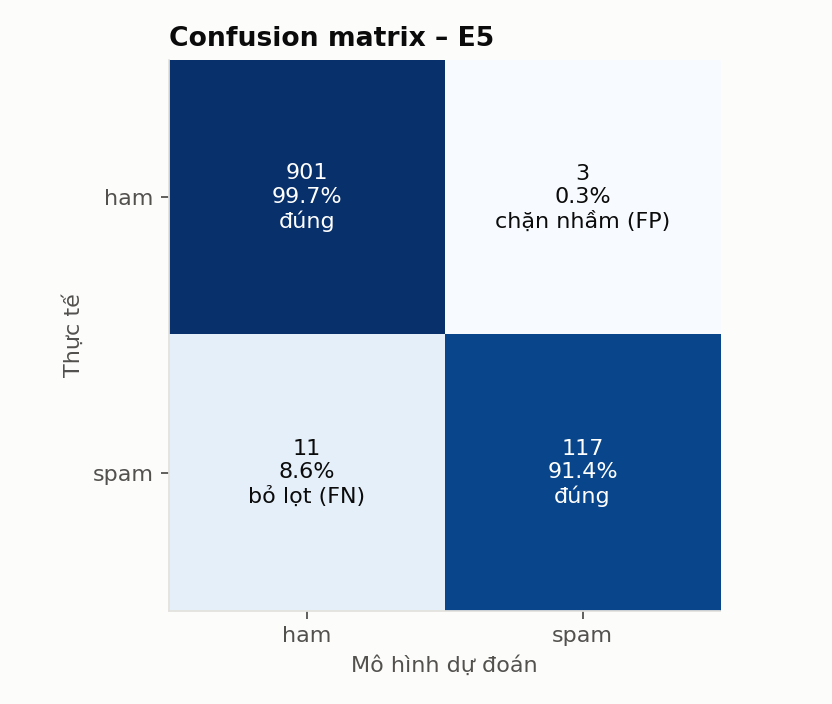
\includegraphics[width=0.6\textwidth]{images/viz_5_confusion_matrix.png}
    \caption{Ma trận nhầm lẫn của E5 trên tập kiểm tra (1\,032 tin)}
    \label{fig:cm-e5}
    \Nguon{Nhóm xây dựng từ kết quả thí nghiệm}
\end{figure}

\section*{Phụ lục 3. Khai báo sử dụng công cụ trí tuệ nhân tạo}

\begin{table}[H]
\centering
\caption{Khai báo sử dụng AI}
\label{tab:ai}
\small
\begin{tabular}{|>{\raggedright\arraybackslash}p{2.4cm}|>{\raggedright\arraybackslash}p{3.6cm}|>{\raggedright\arraybackslash}p{3.4cm}|>{\raggedright\arraybackslash}p{4cm}|}
\hline
\textbf{Công cụ} & \textbf{Mục đích} & \textbf{Phần liên quan} & \textbf{Nhóm đã kiểm tra/chỉnh sửa} \\
\hline
Claude Code & Dựng khung mã nguồn và hướng dẫn làm bài & Thư mục \texttt{spam\_filter/}, tệp \texttt{HUONG\_DAN\_} \texttt{LAM\_BAI.md} & \textit{(nhóm điền: cách kiểm tra, chạy lại và chỉnh sửa)} \\
\hline
Claude Code & Soạn thảo mã nguồn LaTeX của báo cáo từ kết quả thực nghiệm và mẫu báo cáo & Thư mục \texttt{reports/} & \textit{(nhóm điền: đối chiếu số liệu với \texttt{outputs/results/}, chỉnh sửa nội dung)} \\
\hline
\end{tabular}
\Nguon{Nhóm khai báo; xem thêm tệp \texttt{AI\_USAGE.md}}
\end{table}

\section*{Phụ lục 4. Phân công công việc}

\begin{table}[H]
\centering
\caption{Phân công công việc của nhóm}
\label{tab:phan-cong}
\begin{tabular}{|c|p{3.6cm}|p{4cm}|p{3.8cm}|}
\hline
\textbf{STT} & \textbf{Họ và tên} & \textbf{Mã sinh viên} & \textbf{Nhiệm vụ} \\
\hline
1 & \textit{(điền)} & \textit{(điền)} & \textit{(điền)} \\
\hline
2 & \textit{(điền)} & \textit{(điền)} & \textit{(điền)} \\
\hline
3 & \textit{(điền)} & \textit{(điền)} & \textit{(điền)} \\
\hline
\end{tabular}
\Nguon{Nhóm tổng hợp}
\end{table}


\clearpage
\UnnumberedChapter{DANH MỤC TÀI LIỆU THAM KHẢO}

\section*{Tiếng Việt}

\begin{enumerate}[series=refs, label={[\arabic*]}, leftmargin=1.27cm]
    \item\label{bib:tiep2018} Vũ Hữu Tiệp. (2018). \textit{Machine Learning cơ bản}. Truy cập tại \url{https://machinelearningcoban.com}.
\end{enumerate}

\section*{Tiếng Anh}

\begin{enumerate}[resume*=refs, label={[\arabic*]}, leftmargin=1.27cm]
    \item\label{bib:almeida2011} Almeida, T. A., Gómez Hidalgo, J. M., \& Yamakami, A. (2011). Contributions to the study of SMS spam filtering: new collection and results. \textit{Proceedings of the 11th ACM Symposium on Document Engineering (DocEng '11)}, 259--262.
    \item\label{bib:uci_sms} Almeida, T. A., \& Gómez Hidalgo, J. M. (2012). \textit{SMS Spam Collection} [Dataset]. UCI Machine Learning Repository. \url{https://archive.ics.uci.edu/dataset/228/sms+spam+collection}.
    \item\label{bib:scikit-learn} Pedregosa, F., Varoquaux, G., Gramfort, A., et al. (2011). Scikit-learn: Machine learning in Python. \textit{Journal of Machine Learning Research}, 12, 2825--2830.
    \item\label{bib:manning2008} Manning, C. D., Raghavan, P., \& Schütze, H. (2008). \textit{Introduction to Information Retrieval}. Cambridge University Press.
    \item\label{bib:mccallum1998} McCallum, A., \& Nigam, K. (1998). A comparison of event models for Naive Bayes text classification. \textit{AAAI-98 Workshop on Learning for Text Categorization}, 41--48.
    \item\label{bib:rennie2003} Rennie, J. D. M., Shih, L., Teevan, J., \& Karger, D. R. (2003). Tackling the poor assumptions of Naive Bayes text classifiers. \textit{Proceedings of the 20th International Conference on Machine Learning (ICML)}, 616--623.
    \item\label{bib:sparckjones1972} Spärck Jones, K. (1972). A statistical interpretation of term specificity and its application in retrieval. \textit{Journal of Documentation}, 28(1), 11--21.
    \item\label{bib:numpy2020} Harris, C. R., Millman, K. J., van der Walt, S. J., et al. (2020). Array programming with NumPy. \textit{Nature}, 585, 357--362.
    \item\label{bib:pandas2010} McKinney, W. (2010). Data structures for statistical computing in Python. \textit{Proceedings of the 9th Python in Science Conference}, 56--61.
    \item\label{bib:matplotlib2007} Hunter, J. D. (2007). Matplotlib: A 2D graphics environment. \textit{Computing in Science \& Engineering}, 9(3), 90--95.
\end{enumerate}


\end{document}
